\chapter[Order and Disorder in Procrystalline Lattices]{Order and Disorder in \\ Procrystalline Lattices} 

\begin{chapterabstract}
Recent work has introduced the term ``procrystalline'' to define systems which lack translational symmetry but have an underlying high symmetry lattice, owing to a difference between the coordination numbers of the molecular units and the underlying lattice.
These materials are expected to lie between crystalline and amorphous phases.
The network properties of a range of these procrystals are investigated, encompassing a range of coordination environments.
Configurations are generated using a zero\--temperature \mc{} method, whilst simpler lattices are also considered analytically.
Procrystals are shown to be rare examples of systems with violate \lm{}'s law, whilst also displaying assortativities different to those calculated for amorphous materials.
Procrystalline lattices are therefore shown to have fundamentally different behaviour to traditional disordered and crystalline systems, indicative of the partial ordering of the underlying lattices.
\end{chapterabstract}

\section{The Procrystalline State}

Investigations into inorganic network\--forming materials have led to the introduction of the term ``procrystalline'' to refer to systems in which molecular building blocks lie on a regular array of lattice points, but directional interactions lead to overall correlated disorder \cite{Overy2016}.
As an introductory example, consider the procrystal in figure \ref{fig:prointroa}.
In this configuration the nodes form a square net, but each lattice site is occupied by a ``T'' shaped unit.
If the ends of these units are mutually attractive, they will orient to maximise favourable interactions.
The consequence of this is to introduce disorder into the ring structure.
This can be detected in the dual network, as in figure \ref{fig:prointrob}, which in this case can be viewed as a defective square net.
More strikingly, a system of percolating rings once again emerges, highlighted in figure \ref{fig:prointroc}, in analogue with networks from previous chapters. 

\begin{figure}[bt]
     \centering
     
     \begin{subfigure}[b]{0.3\textwidth}
         \centering
         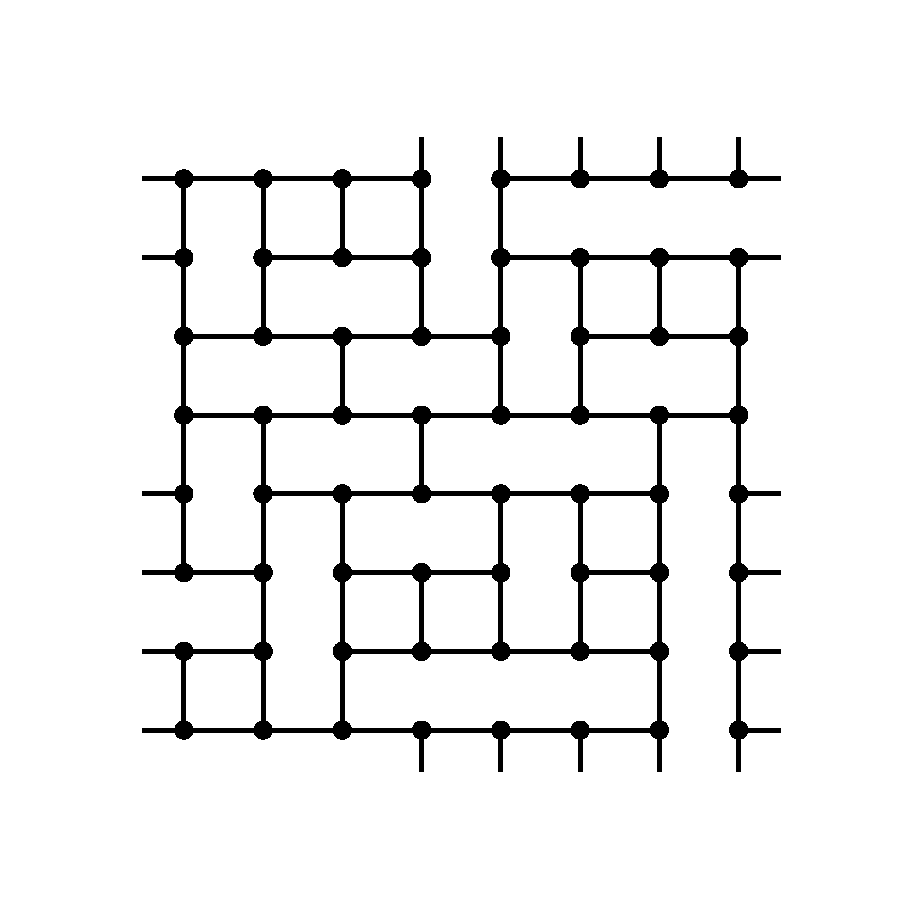
\includegraphics[width=\textwidth]{./figures/procrystals/pro_intro3.pdf}
         \caption{Procrystalline lattice}
         \label{fig:prointroa}
     \end{subfigure}
     \hfill
      \begin{subfigure}[b]{0.3\textwidth}
         \centering
         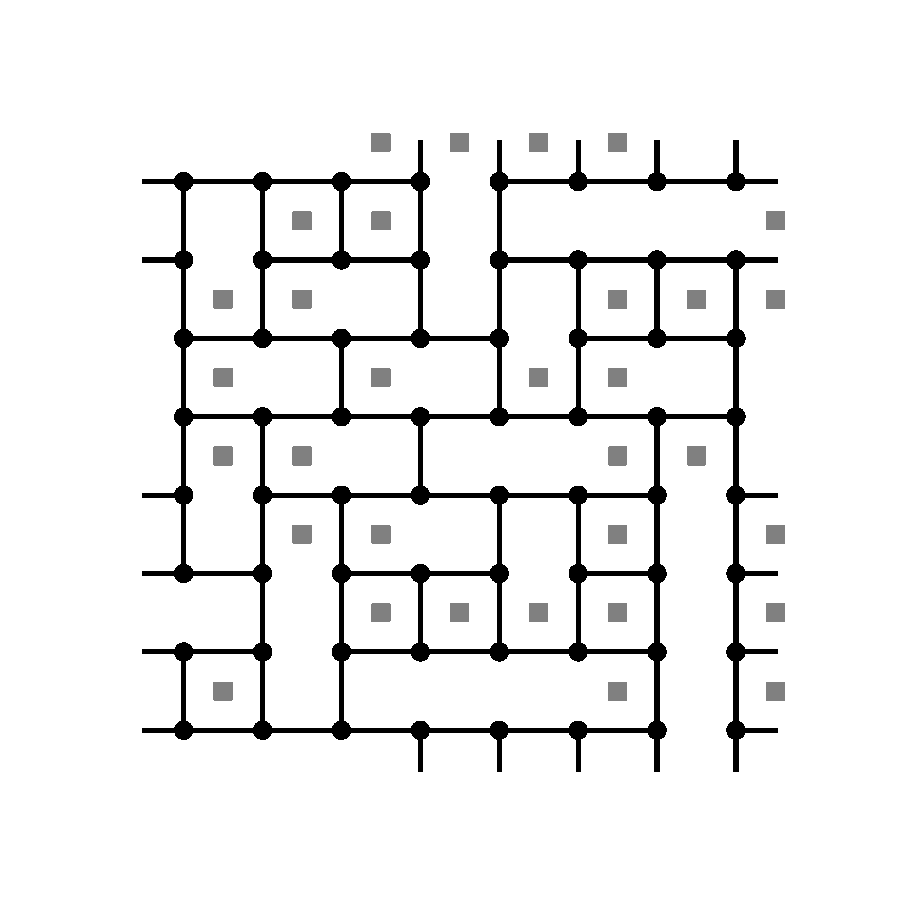
\includegraphics[width=\textwidth]{./figures/procrystals/pro_intro1.pdf}
         \caption{Overlay with dual}
         \label{fig:prointrob}
     \end{subfigure}
     \hfill
     \begin{subfigure}[b]{0.3\textwidth}
         \centering
         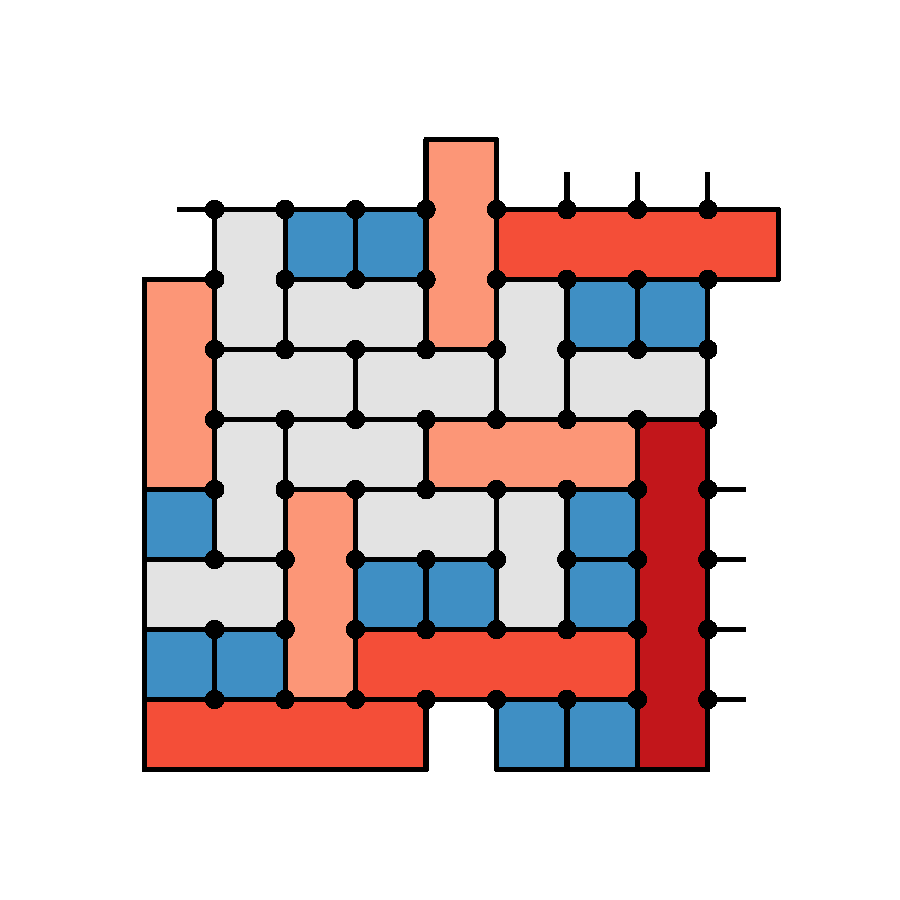
\includegraphics[width=\textwidth]{./figures/procrystals/pro_intro2.pdf}
         \caption{Ring structure}
         \label{fig:prointroc}
     \end{subfigure}
     
     \caption{Example procrystalline lattice based on the square net. Panel (a) shows the lattice with each node representing a 3\--coordinate molecular unit. Panel (b) adds the nodes of the dual network, which form a defective square lattice. Panel (c) highlights the corresponding ring structure, coloured by ring size.}
     \label{fig:nprointro}
\end{figure}

The local environment around each node in a procrystal is therefore identical, leading them to appear crystalline in their atomic RDFs and structure factors. 
However, considering the network in its entirety with both nodes and links, it is clear an infinite procrystalline lattice has no unit cell.
As such procrystals can be considered to sit somewhere in between traditional crystals and the amorphous materials discussed in previous chapters.
This ``partial disordering'' is expected to be reflected in their structural and electronic properties.

Experimentally there are several systems which can be thought of as realisations of procrystals. 
These include self-assembled molecular monolayers, classical bond valence solids, mixed-anion perovskites, and order/disorder ferroelectrics \cite{Blunt2008,Anderson1973,Camp2012,Comes1968}.
Whilst this list is not extremely extensive (particularly for \td{} examples), it demonstrates the diversity in the range of potential structures that can form procrystals.
Again although the future focus of the field may be lie more in three\--dimensional structures, the constraints and simplifications that arise from reduced dimensionality make \td{} structures the natural starting place for investigations into the properties of these procrystalline materials.

\section{Two\--Dimensional Procrystalline Lattices}

In this chapter a range of \td{} procrystalline systems will be investigated based on a selection of underlying high symmetry lattices and node coordination numbers.
Figure \ref{fig:symlat} details the high symmetry lattices that form the basis of these procrystals.
These regular and semi\--regular tilings have been chosen to provide a series of underlying coordination numbers in the range $4\rightarrow6$, whilst also occurring across various theoretical and experimental studies on \td{} materials.
The $4$\--coordinate tilings considered are the square \cite{Algara-Siller2015,Zhu2017,Hibble2011} and trihexagonal (also known as kagome) \cite{Zheng2014,Postulka2016,Chen2011} nets,
the $5$\--coordinate tilings are the elongated\--triangular \cite{Griffith2018} and snub\--square \cite{Urgel2014,Kryuchkov2018,Song2015,Pineros2016} nets, and the $6$\--coordinate tiling is the triangular net. 

\begin{figure}[bt]
     \centering
     
     \begin{subfigure}[b]{0.3\textwidth}
         \centering
         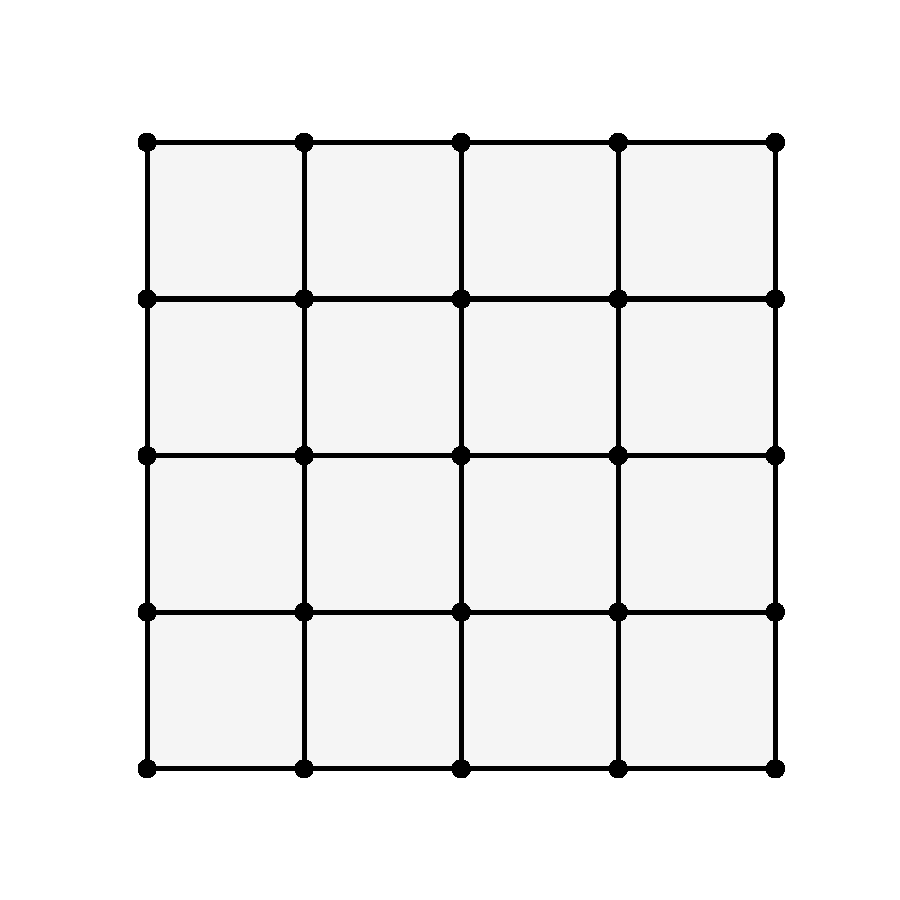
\includegraphics[height=2.5cm]{./figures/procrystals/sq.pdf}
         \caption{Square}
         \label{fig:symlatsq}
     \end{subfigure}
     \begin{subfigure}[b]{0.3\textwidth}
         \centering
         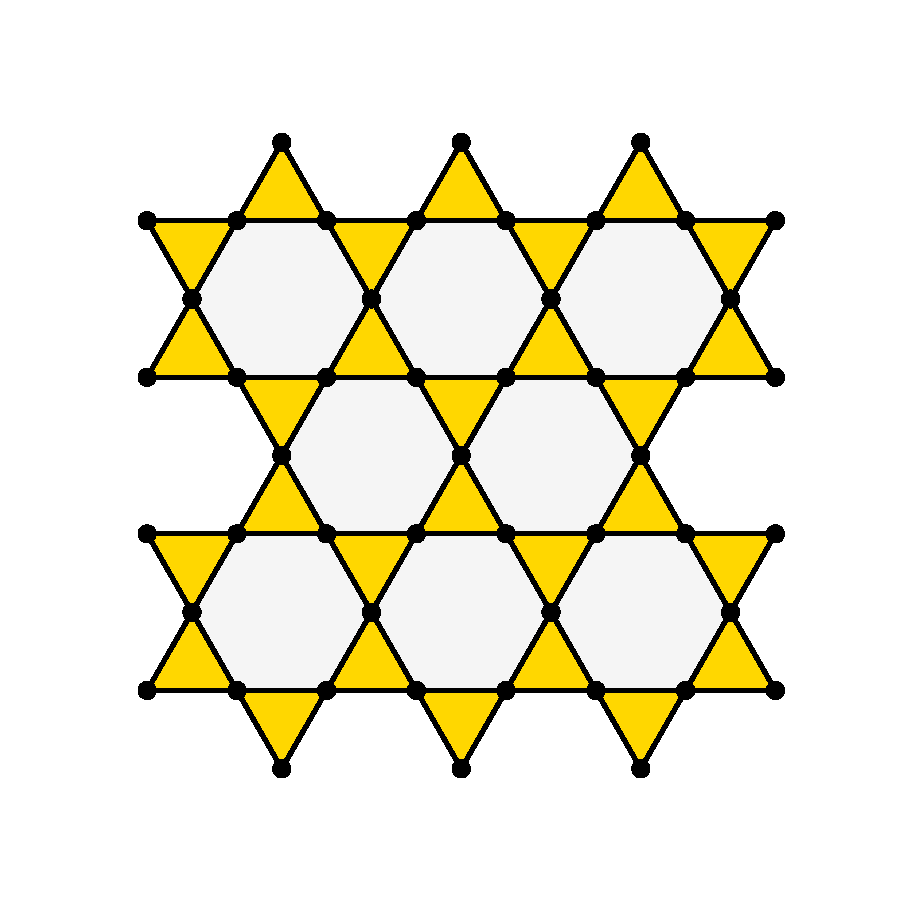
\includegraphics[height=2.5cm]{./figures/procrystals/trihex.pdf}
         \caption{Trihexagonal (kagome)}
         \label{fig:symlattrihex}
     \end{subfigure}
     \hfill
     
     \vspace{0.5cm}
     
     \begin{subfigure}[b]{0.3\textwidth}
         \centering
         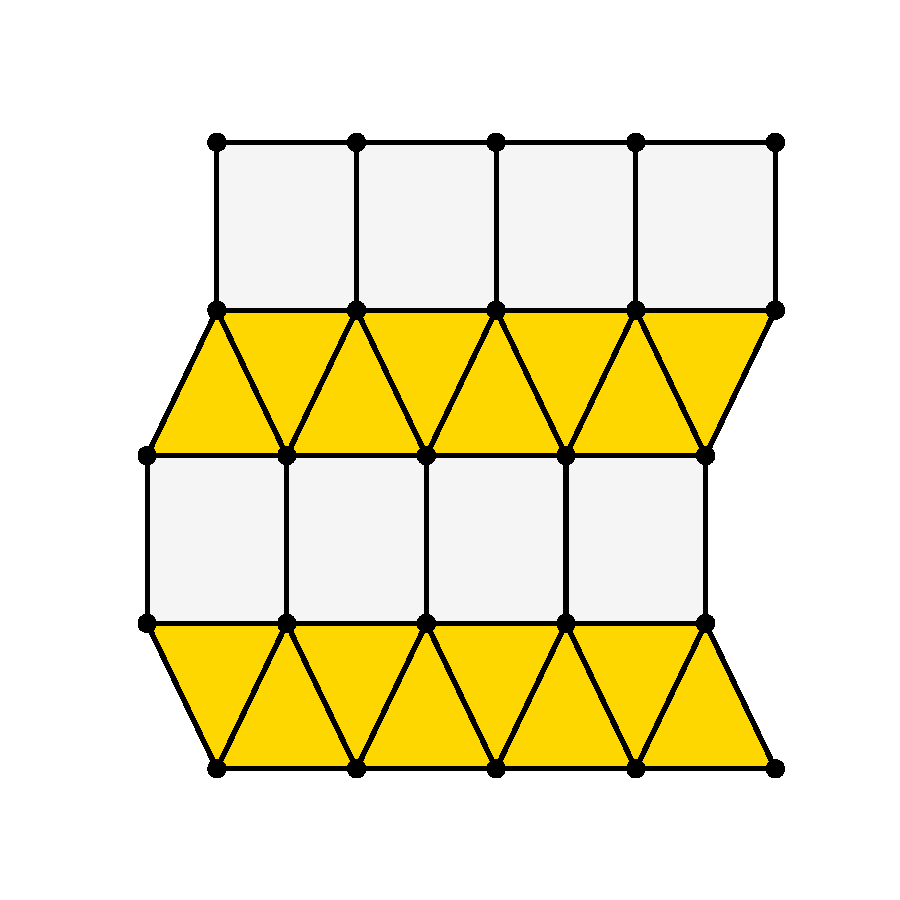
\includegraphics[height=2.5cm]{./figures/procrystals/elongtri.pdf}
         \caption{Elongated\--triangular}
         \label{fig:symlatelong}
     \end{subfigure}
     \hfill
     \begin{subfigure}[b]{0.3\textwidth}
         \centering
         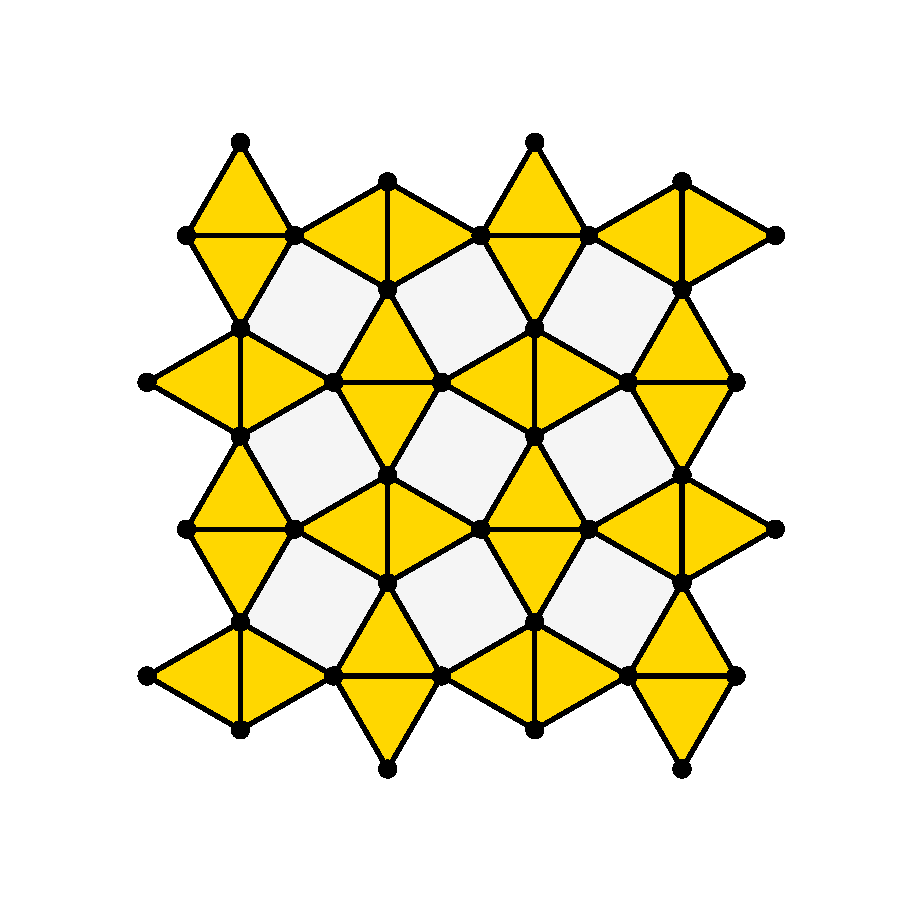
\includegraphics[height=2.5cm]{./figures/procrystals/snub.pdf}
         \caption{Snub\--square}
         \label{fig:symlatsnub}
     \end{subfigure}
     \hfill
     \begin{subfigure}[b]{0.3\textwidth}
         \centering
         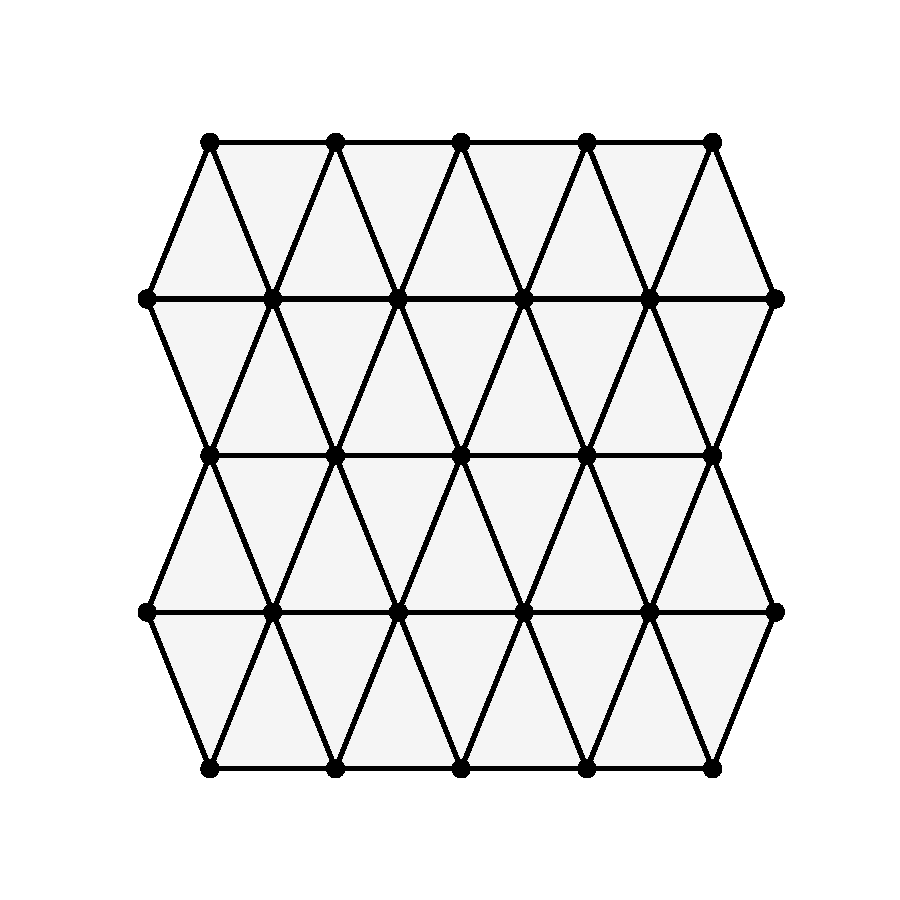
\includegraphics[height=2.5cm]{./figures/procrystals/tri.pdf}
         \caption{Triangular}
         \label{fig:symlattri}
     \end{subfigure}
     \hfill

     \caption{High symmetry lattices that form the basis of \td{} procrystalline lattices in this work. The square and trihexagonal lattices (panels (a), (b)) have a natural coordination number of 4; the elongated triangular and snub square lattices (panels (c), (d))  of 5 and the triangular lattice (panel (e)) of 6.}
     \label{fig:symlat}
\end{figure}

The disorder in procrystals arises from the discrepancy between the natural coordination numbers of the regular lattice and the actual coordination of the nodes which occupy them.
If the node coordination of these high symmetry ``parent'' lattices is denoted $c^\prime$, it follows that each is is able to generate procrystalline lattices with node coordinations, $c$, in the range $c=3\rightarrow \left(c^\prime-1\right)$ (strictly 2\--coordinate procrystals are also obtainable, but these form ``spaghetti'' like structures with ill defined ring structure \cite{Baise2018}).
In this thesis, for simplicity these procrystals will be referred to with the notation \pro{c^\prime}{c}lattices.
In addition, whilst for \pro{c^\prime}{\left(c^\prime-1\right)}lattices there is only one possible way of arranging the $c^\prime-1$ links around each node, for the other lattices this is not the case.
As a simplification it will be assumed that all arrangements are possible and equally likely.

\subsection{Network Measures}

Procrystals can be considered as additional examples of the tessellating ring structures seen in previous chapters, the difference being that the ring geometries are constrained by the underlying lattice. 
As such the network measures discussed previously are also applicable to procrystalline lattices.  
For instance, procrystals are subject to Euler's formula such that the mean ring size is constrained by equation \eqref{eq:avdegree}.

When discussing the maximum entropy ring size distributions, a similar approach can be taken as for \lm's law (see section \ref{s:lemaitre}), save constraint \eqref{con:lm3} no longer applies.
To get the expected maximum entropy ring statistics, $\pme_k$, one can remove this constraint to give a simple modification of equation \eqref{eq:mepk}:
\begin{equation}
    \pme_k = \frac{e^{-\lambda k}}{\sumk e^{-\lambda k}}\,.
\end{equation}
As with \lm's law, an important additional constraint arises implicitly through the $k$\--range in the summation.
Owing to the fact that there are many subtly different systems here, these will be further discussed in the relevant sections \davidnote{link}.

Finally, the assortativity will again be used to measure ring\--ring correlations. \davidnote{ref}

\section{Computational Generation of Procrystals}

Although experimental procrystalline lattices are aperiodic with no unit cell, computational studies are naturally restricted in scope and an effective way of generating lattices with fully satisfied valence is to reintroduce periodicity. 
There are then two possible ways to proceed in order to map the configurational space of procrystals.
Firstly, one can attempt to find all possible arrangements for a lattice of given size, which here is termed \textit{exact tiling}.
Whilst exact tiling gives a complete view of the procrystalline landscape, it will be seen that even with optimisations it quickly becomes computationally intractable.

The second approach is to sample configurations using a stochastic method such as \mc{} sampling.
This allows procrystalline configurations to be generated which are representative of the wider landscape for far larger lattice dimensions.
This has the advantage of mitigating any effects of enforcing periodicity, and will be the primary method used to generate procrystals in this work.

\subsection{Exact Tiling Algorithm}

The exact tiling algorithm finds all periodic procrystalline lattices for a given lattice dimension using a divide\--and\--conquer approach.
It has been used here to investigate the \pro{4}{3}square lattice.
The method starts from the observation that there are seven possibilities for each square in the procrystalline lattice (some of which are symmetry related) forming the $1\times 1$ tiles in figures \ref{fig:et1x1_0}\--\ref{fig:et1x1_6} (these are colour coded by a central circle).
These $1\times 1$ tiles can be stacked to produce $1\times 2$ tiles, of which there are 22 possibilities that satisfy internal coordination requirements (but are not necessarily periodic), the first 5 of which are given in figures \ref{fig:et2x1_0}\--\ref{fig:et2x1_4}.
Again these can in turn be stacked to yield 84 $2\times 2$ building blocks, a selection of which are given in figures \ref{fig:et2x2_0}\--\ref{fig:et2x2p_3}.

\begin{figure}[bt]
     \centering
     
     \begin{subfigure}[b]{0.1\textwidth}
         \centering
         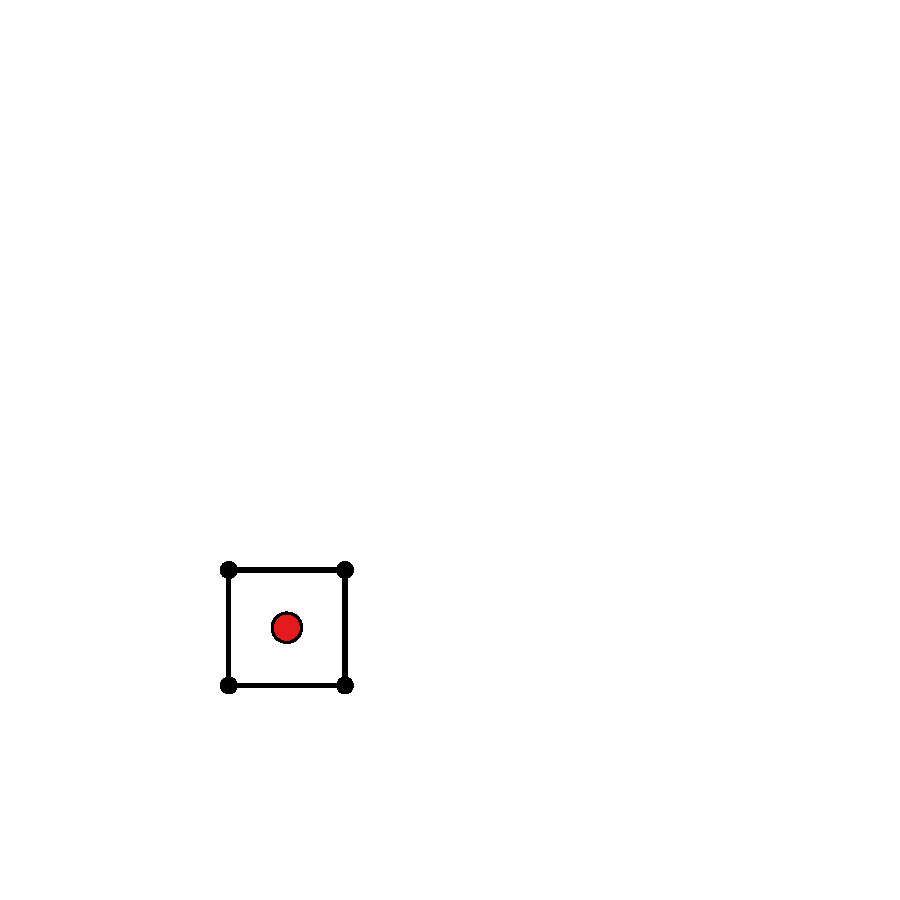
\includegraphics[height=1.2cm]{./figures/procrystals/1x1_0.pdf}
         \caption{}
         \label{fig:et1x1_0}
     \end{subfigure}
     \hfill
     \begin{subfigure}[b]{0.1\textwidth}
         \centering
         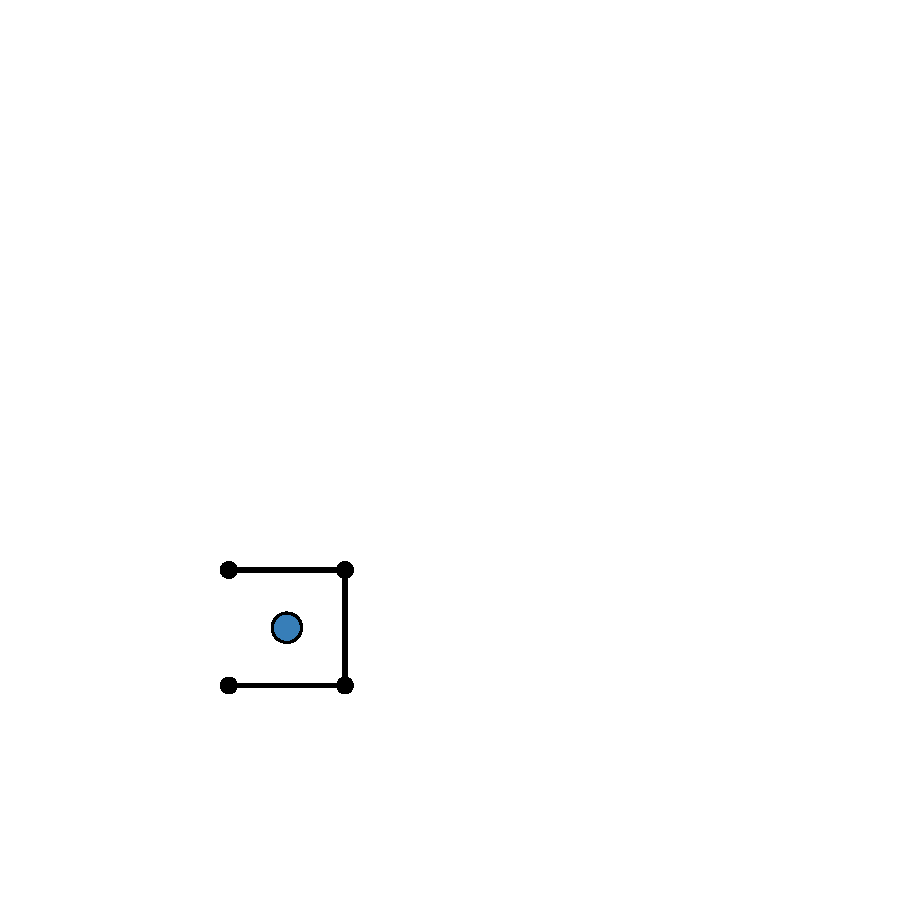
\includegraphics[height=1.2cm]{./figures/procrystals/1x1_1.pdf}
         \caption{}
         \label{fig:et1x1_1}
     \end{subfigure}
     \hfill
     \begin{subfigure}[b]{0.1\textwidth}
         \centering
         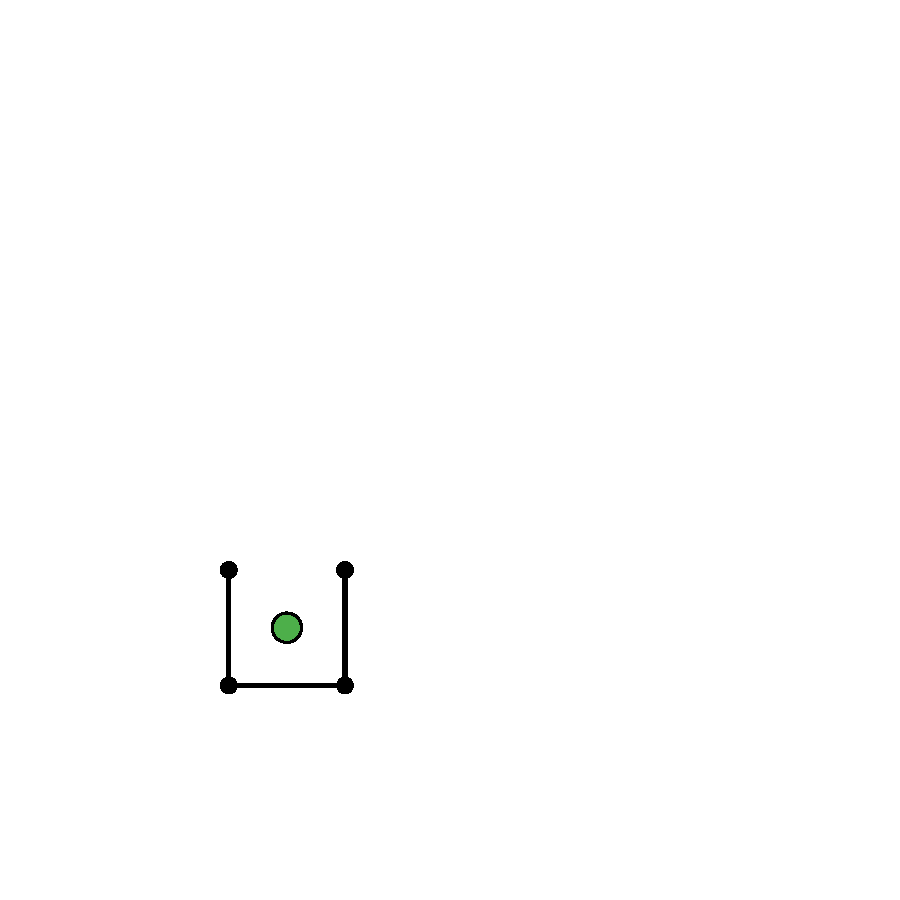
\includegraphics[height=1.2cm]{./figures/procrystals/1x1_2.pdf}
         \caption{}
         \label{fig:et1x1_2}
     \end{subfigure}
     \hfill
     \begin{subfigure}[b]{0.1\textwidth}
         \centering
         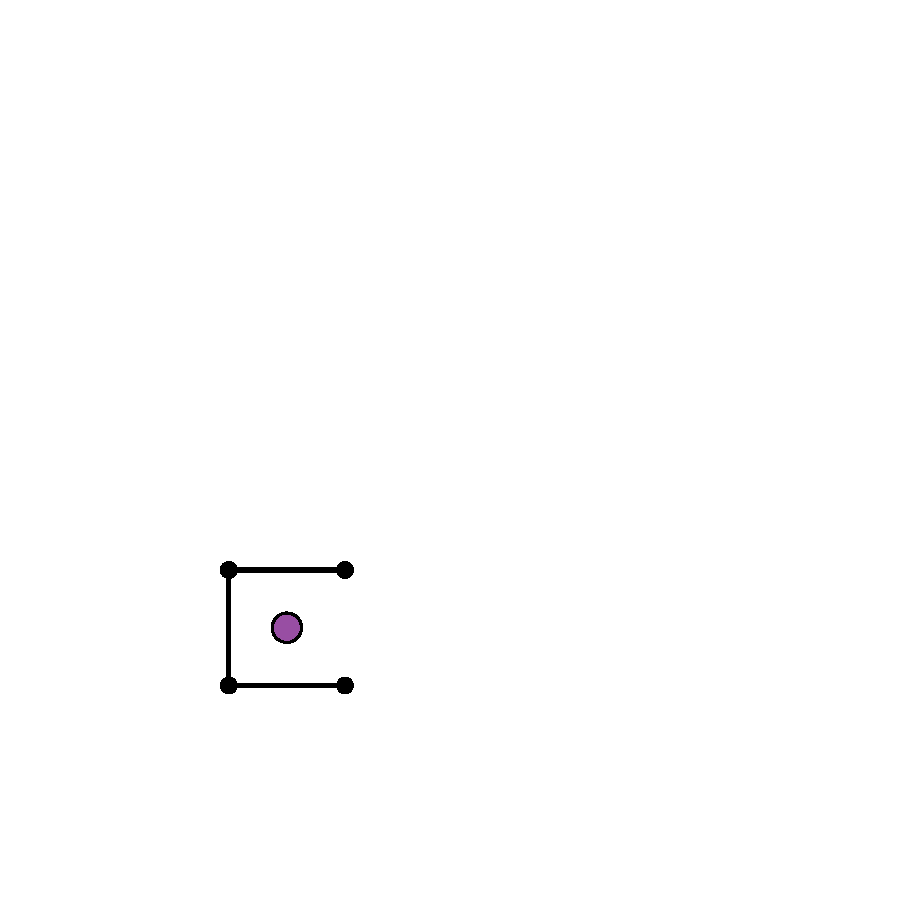
\includegraphics[height=1.2cm]{./figures/procrystals/1x1_3.pdf}
         \caption{}
         \label{fig:et1x1_3}
     \end{subfigure}
     \hfill
     \begin{subfigure}[b]{0.1\textwidth}
         \centering
         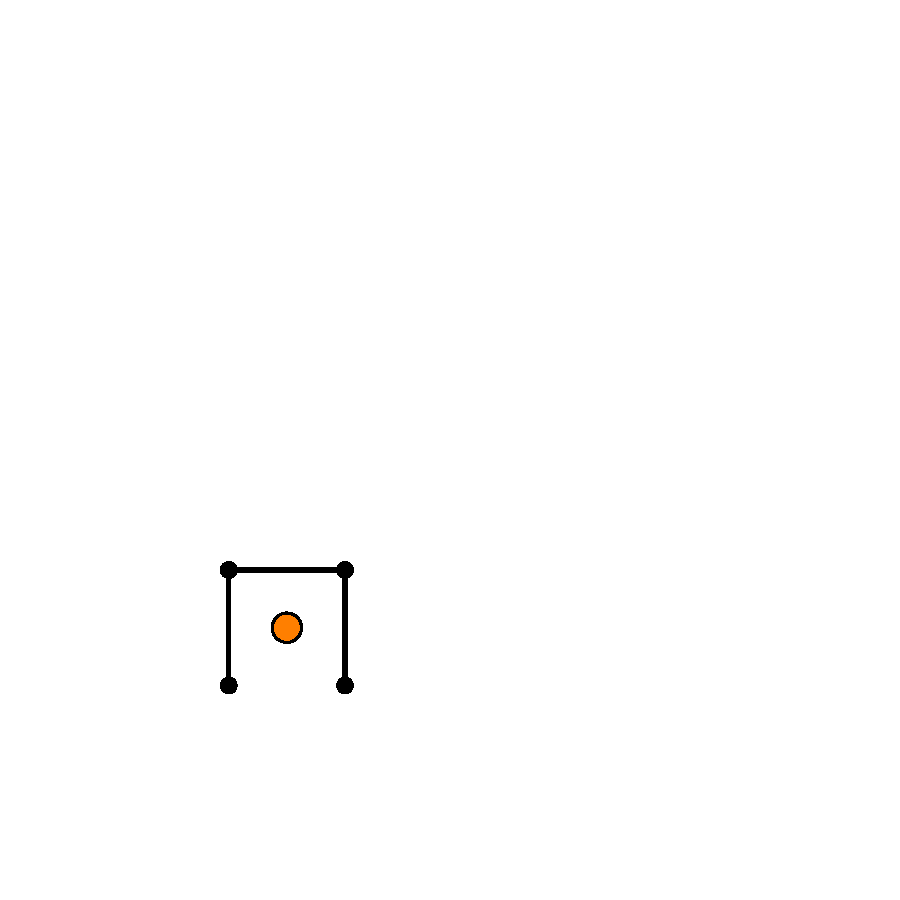
\includegraphics[height=1.2cm]{./figures/procrystals/1x1_4.pdf}
         \caption{}
         \label{fig:et1x1_4}
     \end{subfigure}
     \hfill
     \begin{subfigure}[b]{0.1\textwidth}
         \centering
         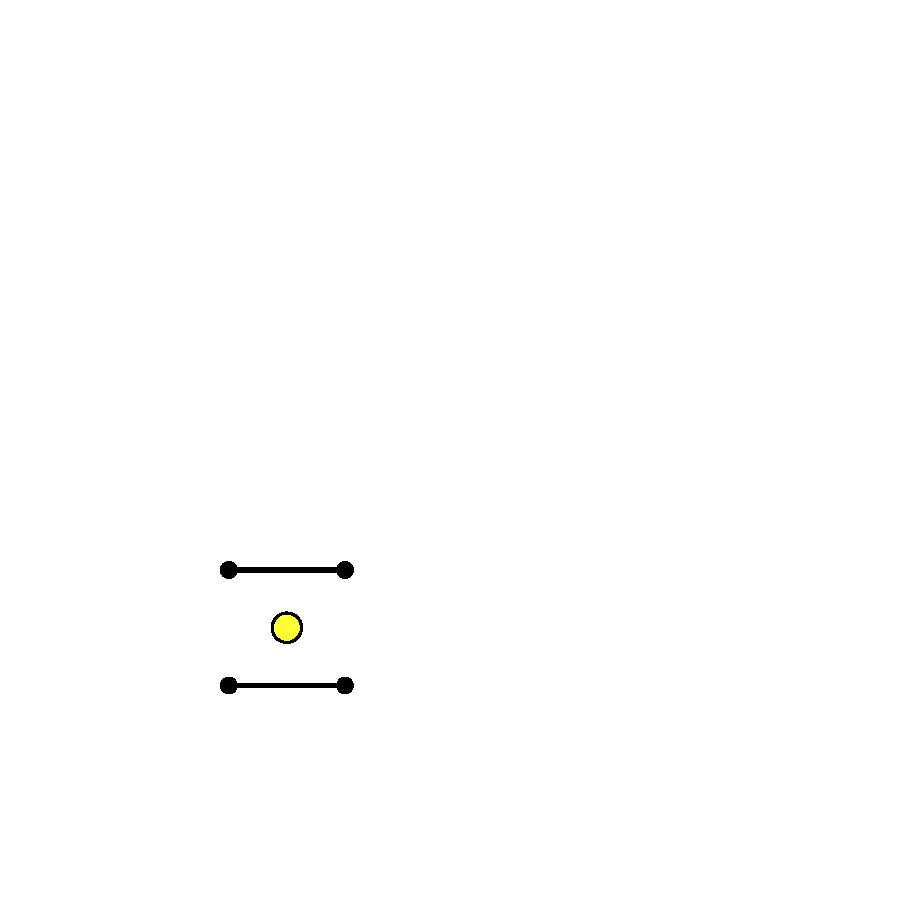
\includegraphics[height=1.2cm]{./figures/procrystals/1x1_5.pdf}
         \caption{}
         \label{fig:et1x1_5}
     \end{subfigure}
     \hfill
     \begin{subfigure}[b]{0.1\textwidth}
         \centering
         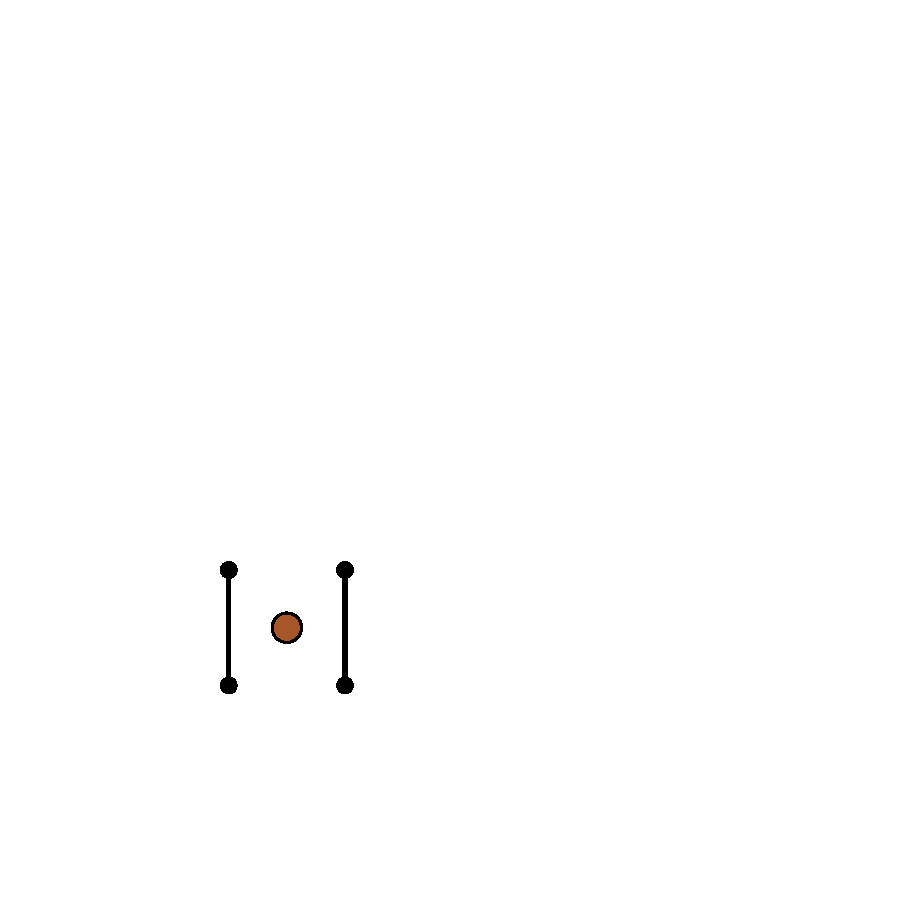
\includegraphics[height=1.2cm]{./figures/procrystals/1x1_6.pdf}
         \caption{}
         \label{fig:et1x1_6}
     \end{subfigure}
     \hfill
     \vspace{0.5cm}
     
     \begin{subfigure}[b]{0.19\textwidth}
         \centering
         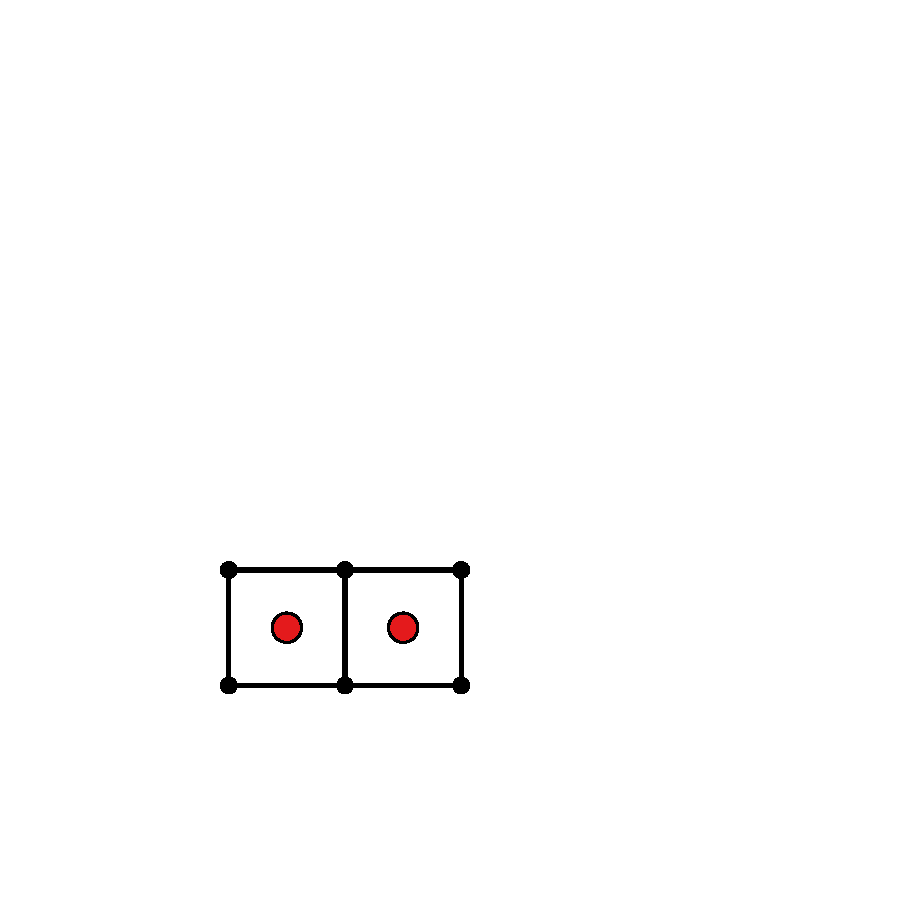
\includegraphics[height=1.2cm]{./figures/procrystals/2x1_0.pdf}
         \caption{}
         \label{fig:et2x1_0}
     \end{subfigure}
     \hfill
     \begin{subfigure}[b]{0.19\textwidth}
         \centering
         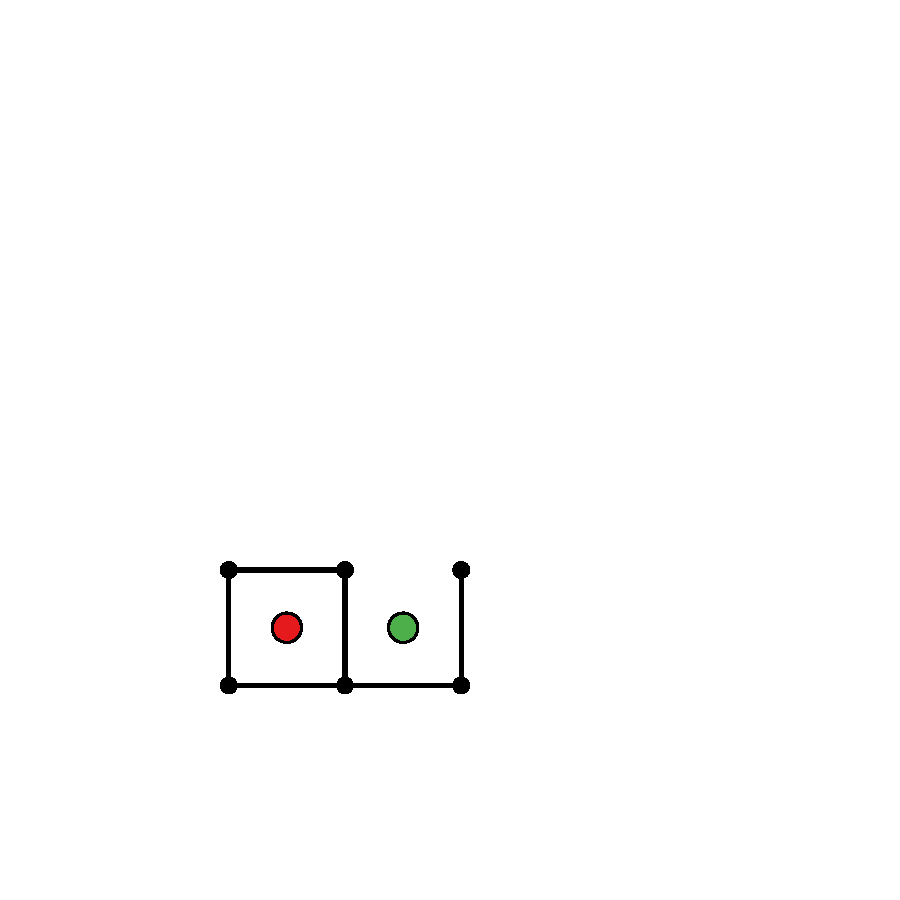
\includegraphics[height=1.2cm]{./figures/procrystals/2x1_1.pdf}
         \caption{}
         \label{fig:et2x1_1}
     \end{subfigure}
     \hfill
     \begin{subfigure}[b]{0.19\textwidth}
         \centering
         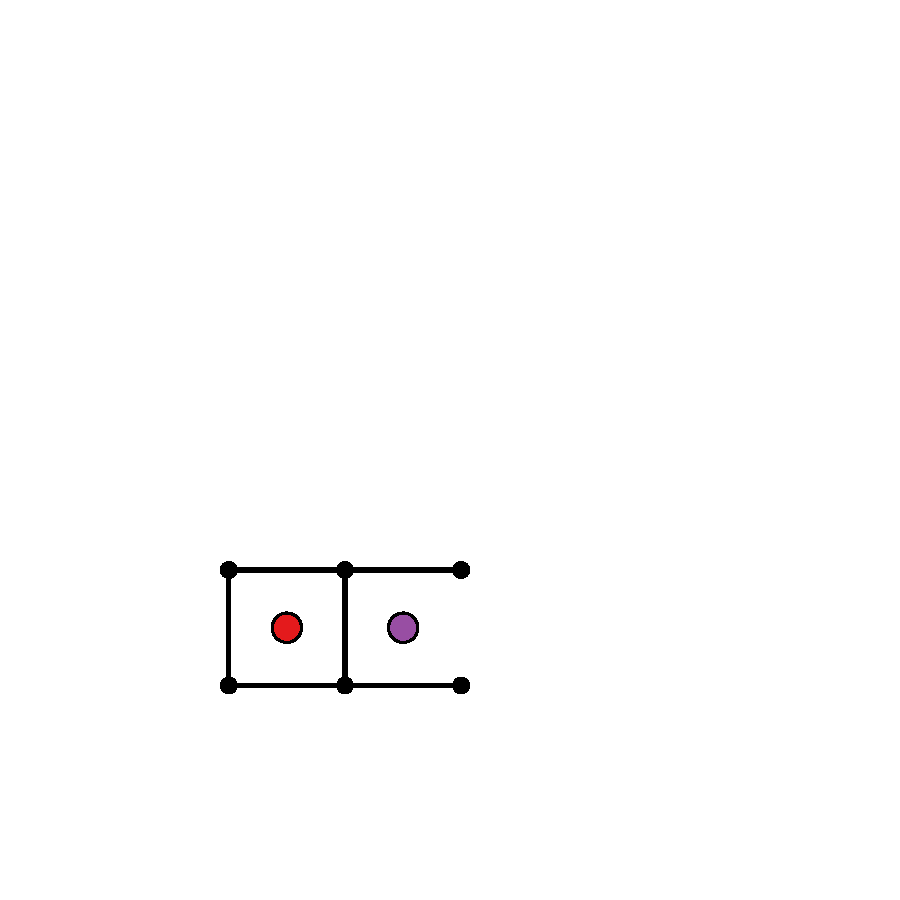
\includegraphics[height=1.2cm]{./figures/procrystals/2x1_2.pdf}
         \caption{}
         \label{fig:et2x1_2}
     \end{subfigure}
     \hfill
    \begin{subfigure}[b]{0.19\textwidth}
         \centering
         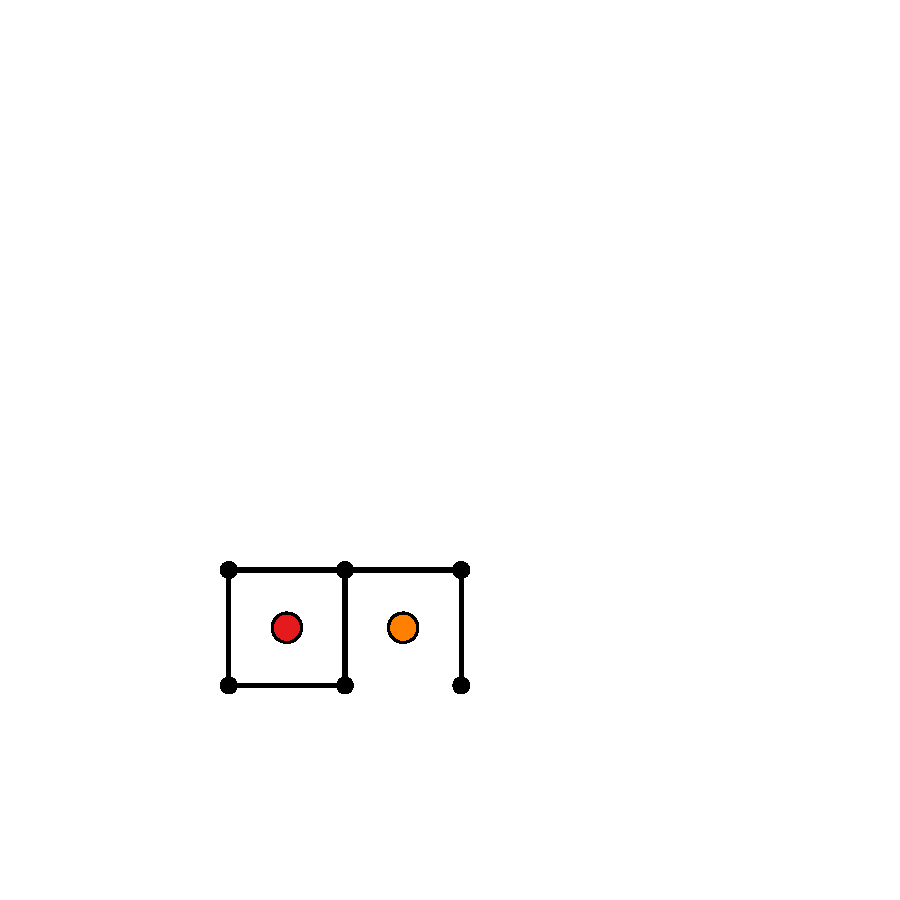
\includegraphics[height=1.2cm]{./figures/procrystals/2x1_3.pdf}
         \caption{}
         \label{fig:et2x1_3}
     \end{subfigure}
     \hfill
    \begin{subfigure}[b]{0.19\textwidth}
         \centering
         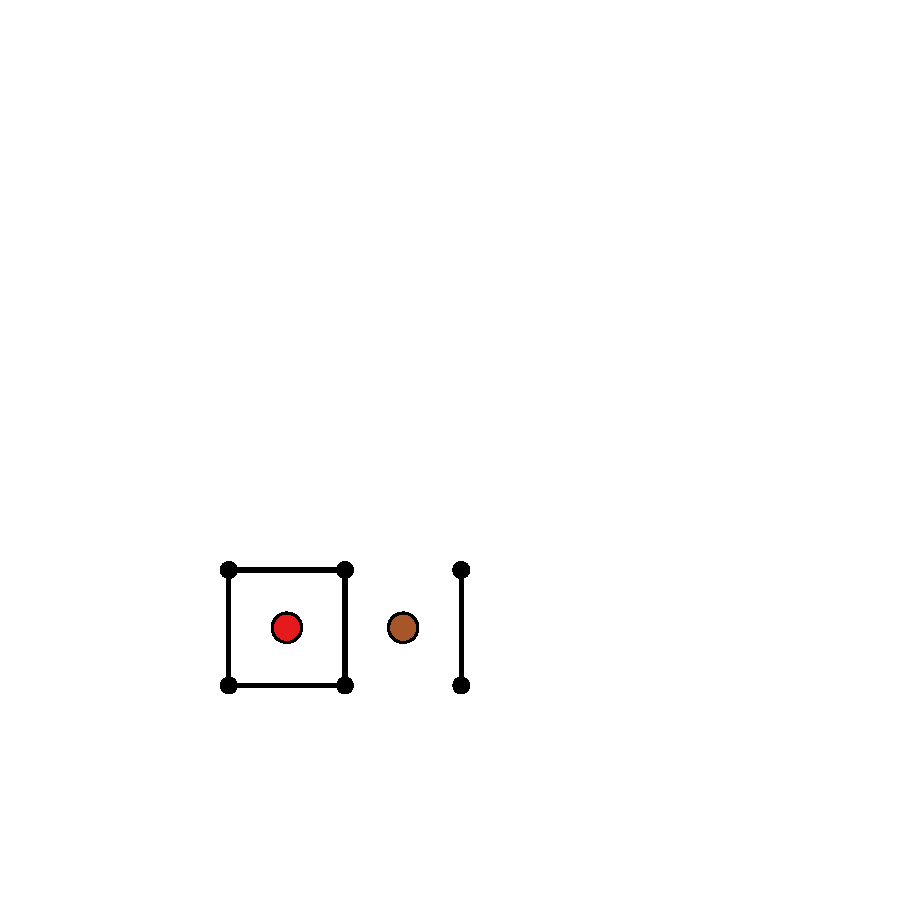
\includegraphics[height=1.2cm]{./figures/procrystals/2x1_4.pdf}
         \caption{}
         \label{fig:et2x1_4}
     \end{subfigure}
     \hfill
	\vspace{0.5cm}     

	\begin{subfigure}[b]{0.19\textwidth}
         \centering
         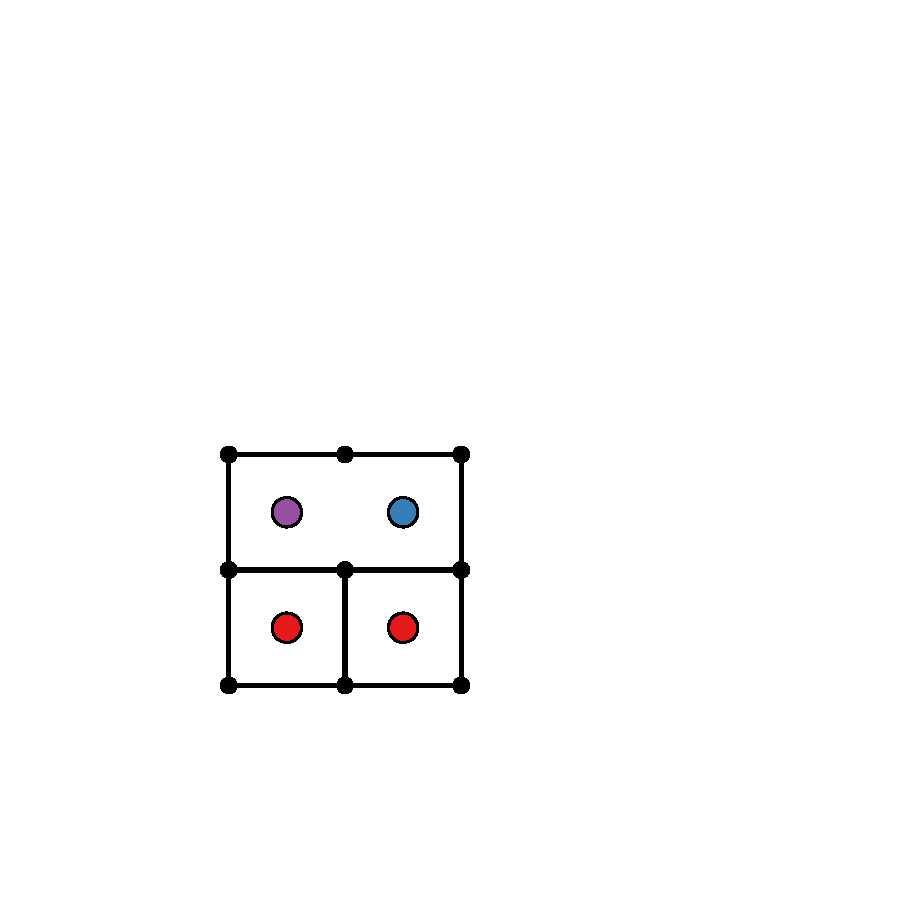
\includegraphics[height=2.2cm]{./figures/procrystals/2x2_10.pdf}
         \caption{}
         \label{fig:et2x2_0}
     \end{subfigure}
     \hfill          
     \begin{subfigure}[b]{0.19\textwidth}
         \centering
         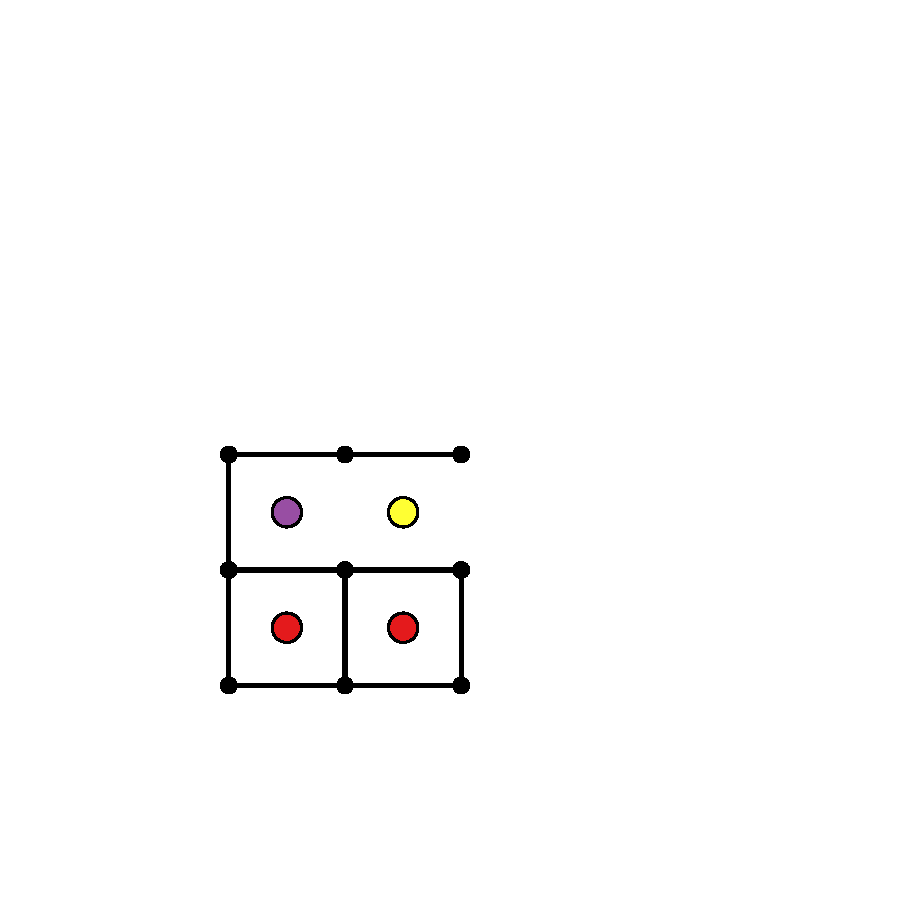
\includegraphics[height=2.2cm]{./figures/procrystals/2x2_11.pdf}
         \caption{}
         \label{fig:et2x2_1}
     \end{subfigure}
     \hfill
     \begin{subfigure}[b]{0.19\textwidth}
         \centering
         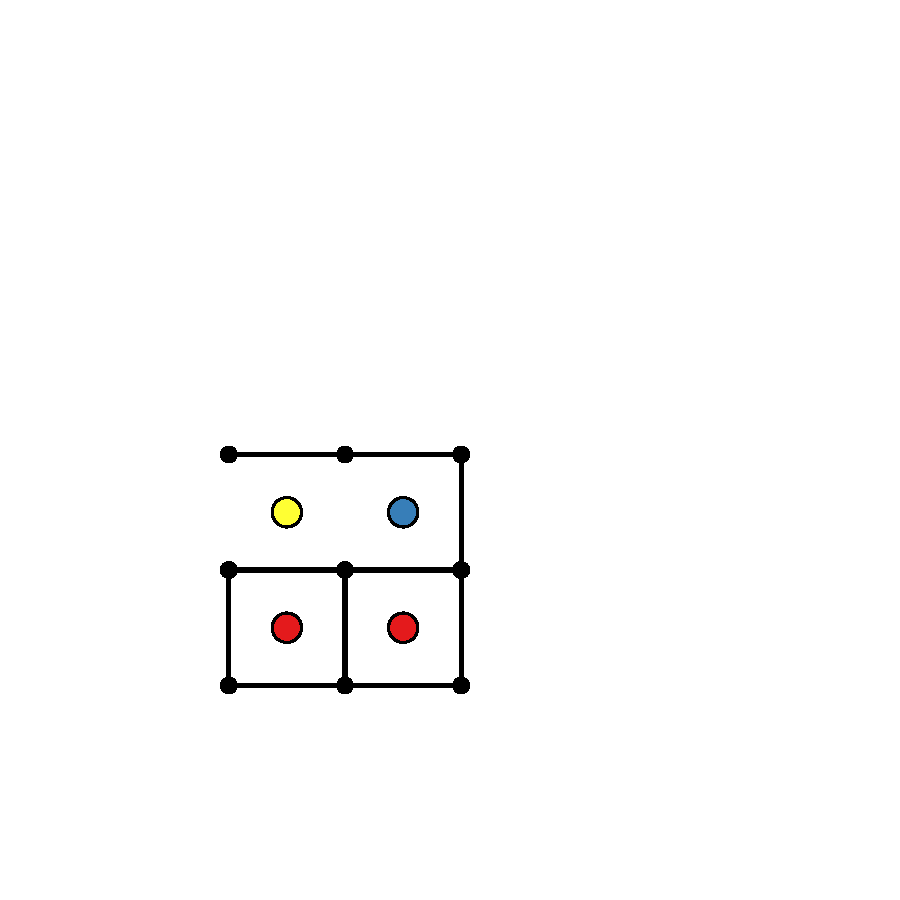
\includegraphics[height=2.2cm]{./figures/procrystals/2x2_15.pdf}
         \caption{}
         \label{fig:et2x2_2}
     \end{subfigure}
     \hfill
     \begin{subfigure}[b]{0.19\textwidth}
         \centering
         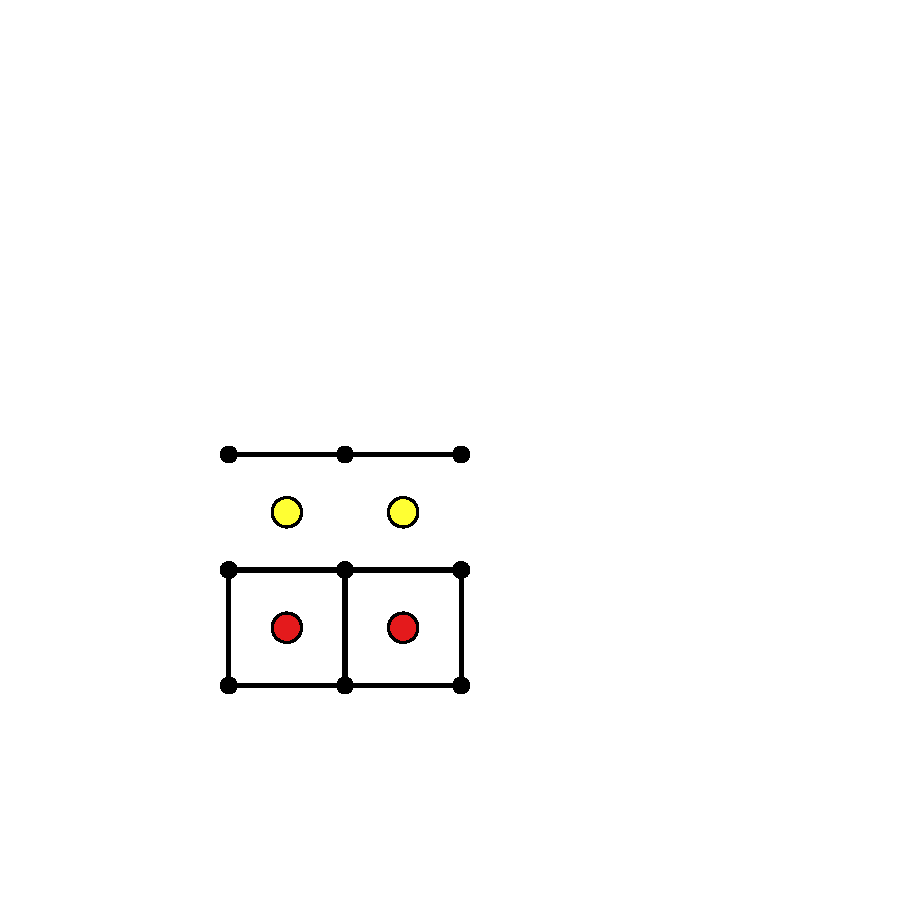
\includegraphics[height=2.2cm]{./figures/procrystals/2x2_16.pdf}
         \caption{}
         \label{fig:et2x2_3}
     \end{subfigure}
     \hfill
	
	\vspace{0.5cm}    
    
     \begin{subfigure}[b]{0.19\textwidth}
         \centering
         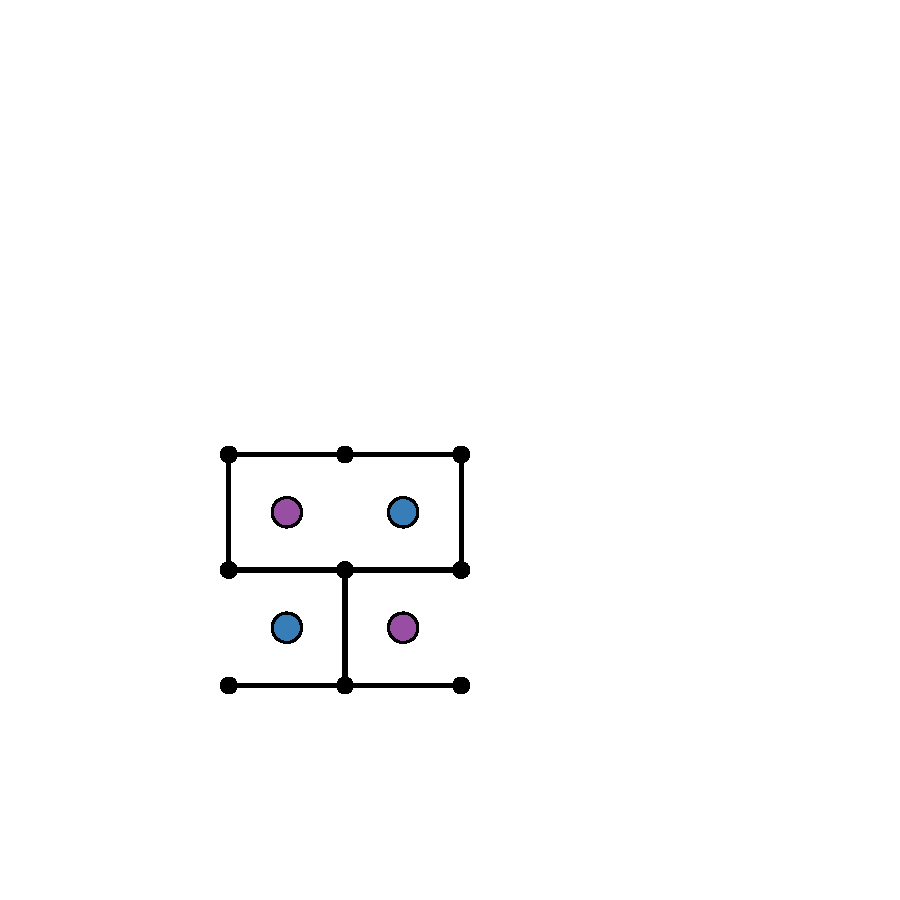
\includegraphics[height=2.2cm]{./figures/procrystals/2x2_0p.pdf}
         \caption{}
         \label{fig:et2x2p_0}
     \end{subfigure}
     \hfill
      \begin{subfigure}[b]{0.19\textwidth}
         \centering
         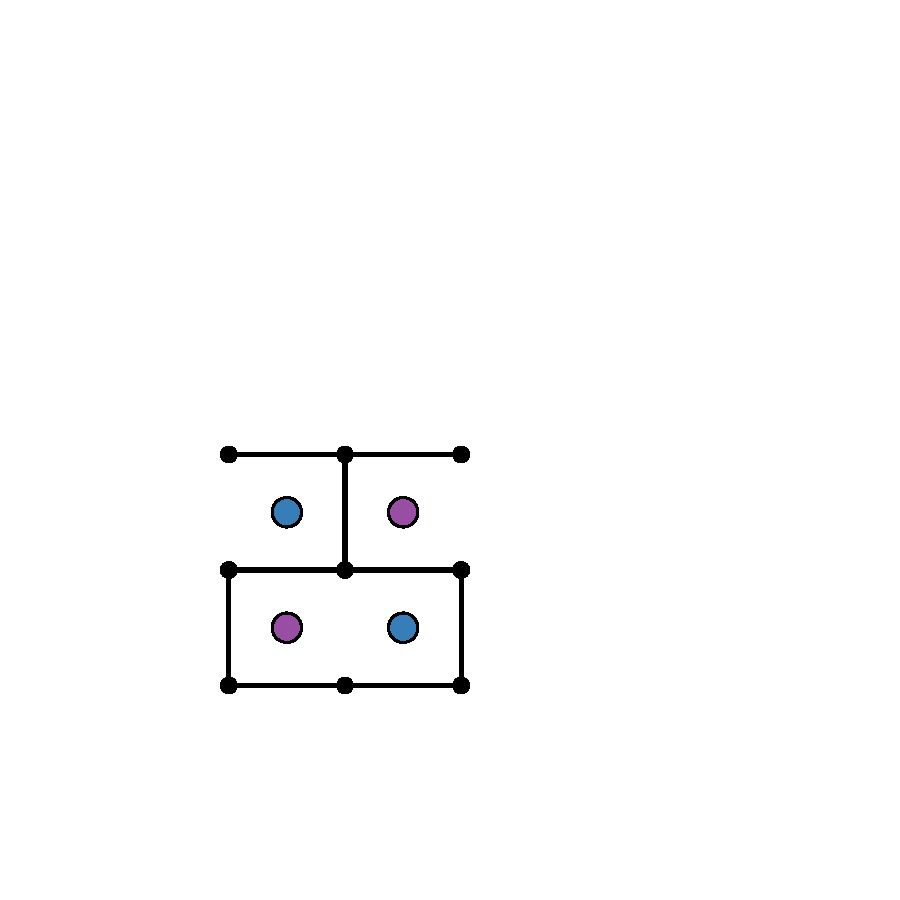
\includegraphics[height=2.2cm]{./figures/procrystals/2x2_2p.pdf}
         \caption{}
         \label{fig:et2x2p_1}
     \end{subfigure}
     \hfill
      \begin{subfigure}[b]{0.19\textwidth}
         \centering
         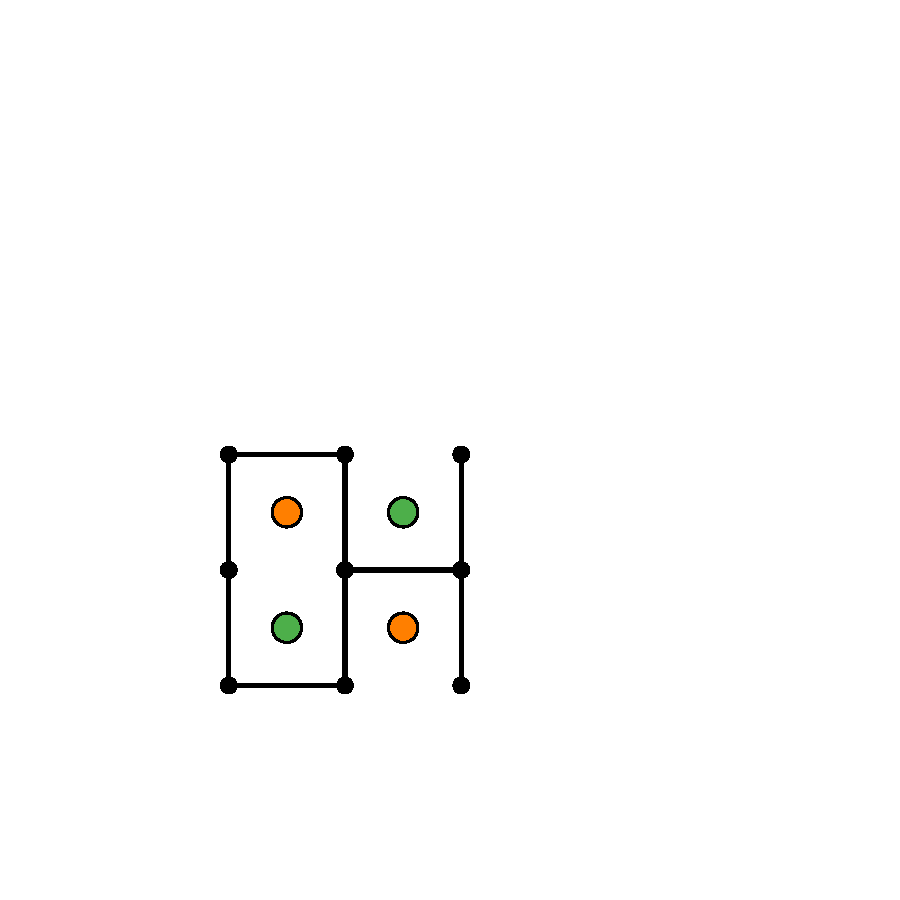
\includegraphics[height=2.2cm]{./figures/procrystals/2x2_1p.pdf}
         \caption{}
         \label{fig:et2x2p_2}
     \end{subfigure}
     \hfill
      \begin{subfigure}[b]{0.19\textwidth}
         \centering
         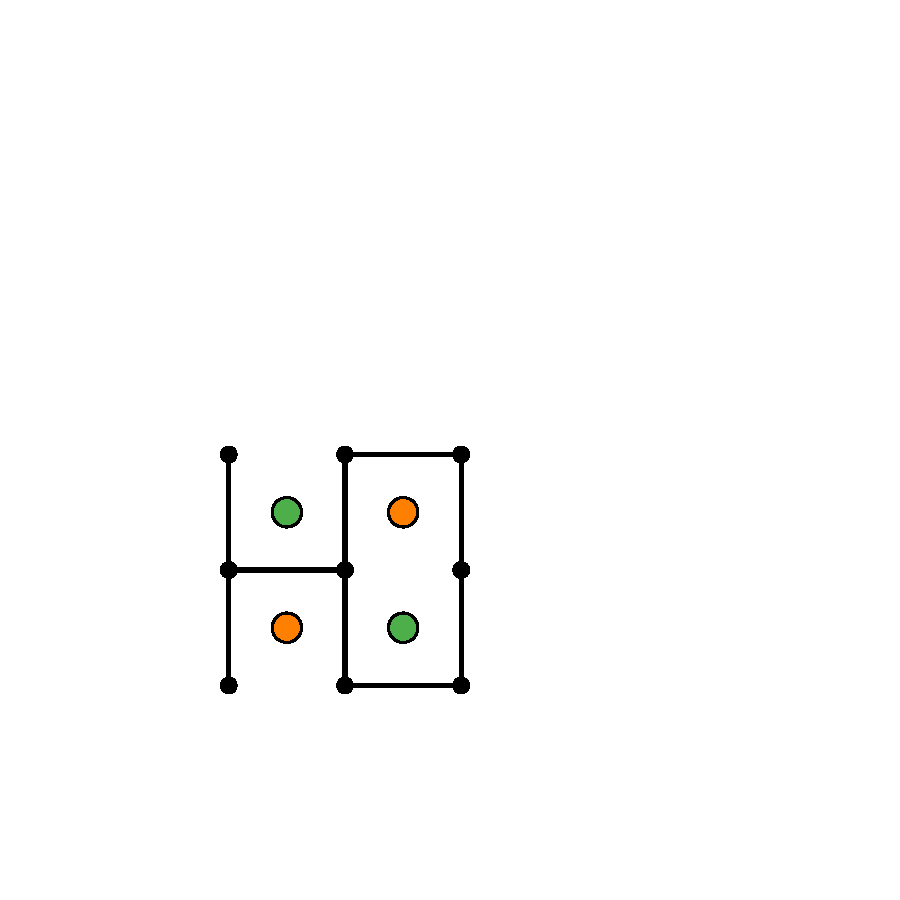
\includegraphics[height=2.2cm]{./figures/procrystals/2x2_3p.pdf}
         \caption{}
         \label{fig:et2x2p_3}
     \end{subfigure}
     \hfill
    
     \caption{Illustration of the process of exact tiling. Panels (a)\--(g) give the 7 fundamental $1\times 1$ environments for a square in the \pro{4}{3}square lattice (individually coloured with a central circle, merely intended a guide for the eye). These can be combined to give $2\times 1$ tiles, the 5 acceptable tiles using (a) shown in panels (h)\--(l). The process can be repeated to build up larger tiles such as the $2\times 2$ tiles in (m)\--(p). Finally the periodic tiles can be identified, the 4 only $2\times 2$ cases given in (q)\--(t).}
     \label{fig:exacttiling}
\end{figure}

It should be clear that this process of combining smaller tiles to form larger tiles can be continued \adinfinitum{}, producing tiles of arbitrary dimension $m\times n$.
This method is vastly more efficient than a brute force search to obtain the same structures, where notionally each ``T'' can adopt 4 positions leading to $4^{m\times n}$ possible configurations - only a fraction of which satisfy the bonding requirements.
The key to the exact tiling method is only to retain units in which the bulk nodes (\ie{} those not on the perimeter) are all 3\--coordinate, thus dramatically reducing the search space.
In order to find the periodic procrystals for a $m\times n$ lattice, one then only has to check for units which can tessellate with $3$\--coordination on the perimeter nodes.
For the $2\times 2$ lattice, only $4 / 84$ of the tiles conform to this rule, shown in figures \ref{fig:et2x2p_0}\--\ref{fig:et2x2p_3}.
It is further evident that these $4$ configurations are all in fact symmetry related, and that the only unique solution is in fact the hexagonal tiling.

The ability to leverage symmetry to reduce the search space further is important when looking at larger lattices. 
This can be achieved by identifying and discarding tiles that are symmetrically equivalent.
Care must be taken however to still form larger tiles by adding the original degenerate set to the reduced set, to avoid losing solutions.
A final improvement can be to check for ``half\--periodicity'' when forming $2m\times n$ tiles from $m\times n$ tiles. 
In this case any units which are not periodic in the fixed dimension can also be discarded before combination takes place.

\begin{table}[bt]
	\centering
     \caption{Performance of the exact tiling algorithm. For each lattice dimension the number of aperiodic, periodic and symmetrically unique periodic tiles are listed. The search space can be found by squaring the number of aperiodic tiles of the previous tile size. }
     \label{tab:exacttiling}
     \begin{tabular}{cccc}
     \toprule
     Lattice & Aperiodic & Periodic & Unique \\
     \midrule
	 $2\times 2$ & 84 & 4 & 1 \\
	 $2\times 4$ & 1,536 & 16 & 4 \\	
	 $2\times 6$ & 27,572 & 64 & 8 \\	
	 %$2\times 8$ & 493,220 & 256 & 18 \\	
	 $4\times 4$ & 87,264 & 204 & 9 \\
	 $4\times 6$ & 4,9147,56 & 2,368 & 70  \\
	 $6\times 6$ & $-$ & 81,736 & 440  \\
     \bottomrule
     \end{tabular}
\end{table}

The application of all the optimisations discussed above serve to make the exact tiling algorithm tractable for a small lattices.
Table \ref{tab:exacttiling} details the performance of the algorithm.
Taking even the $4\times 4$ lattice as an example, a na\"ive search algorithm would require $4^{16}\sim 4\times10^9$ iterations compared to the $1536^2\sim 2\times10^6$ for the exact tiling algorithm.
The difference for the $6\times 6$ lattice becomes even more marked, spanning some 8 orders of magnitude.
However, it is still fighting against the forces of exponential scaling and despite all these improvements in performance, the exact tiling algorithm remains severely limited. 
Table \ref{tab:exacttiling} highlights the enormity of the full configurational space and how small a proportion the procrystal solutions are of the total.
In order to find all the solutions for larger lattices, a more sophisticated algorithm would be required, although it is hard to see how the hurdle of scaling could be easily overcome.

\subsection{Monte Carlo Algorithm}

To generate procrystals for larger lattice dimensions, a method is required that can quickly search configurational space and find representative samples.
As with much of the work in this thesis, this is achieved by utilising a \mc{} algorithm.
The algorithm in question has been developed to produce \pro{c^\prime}{c}lattices of arbitrary size.
It is a zero\--temperature \mc{} algorithm which proceeds as follows:
\begin{enumerate}
	\item Initialise the required $c^\prime$\--coordinate periodic lattice from figure \ref{fig:symlat} and assign each node $c$ bonds in a random orientation. This will introduce a number of dangling bonds into the configuration.
	\item Select a node at random and change the orientation of the bonds.
	\item If the number of dangling bonds is less than or equal to the number in the previous configuration update the configuration; otherwise revert to the previous structure.
	\item Repeat steps 2 and 3 until all dangling bonds have been removed and all node coordinations are satisfied.
	The final lattice is then in the procrystalline state.
\end{enumerate}
This process is demonstrated for an $8\times 8$ \pro{4}{3}square lattice in figure \ref{fig:promc}.
One aspect of note is that as removing the dangling bonds often requires a correlated motion, it becomes increasingly difficult to remove defects as they reduce in number.
Furthermore the structure obtained with a small number of dangling bonds can be quite different to the final procrystalline network as a consequence of the required reorganisation.

This method can be thought of as a simplified version of a site adsorption model, where molecules adsorb to specific sites on an underlying lattice and interact with varying directional potentials \cite{Gorbunov2017,Nieckarz2018,Buzano2004}.
The difference is that here the potential model is binary and the aim of the method is to generate a fully coordinate, defect\--free ``ground state'' procrystalline lattice.
One could in principle introduce a Metropolis type criterion into step 3 (with the the energy difference reflecting the change in number of dangling bonds) and hence accepting a proportion of ``uphill'' moves.
However, the zero\--temperature version is found to converge very well, as there is sufficient flexibility through moves which merely conserve the number of dangling bonds for a global minimum to be reached.
In addition, the temperature parameter was not found to appreciably affect the overall properties of the resulting realisations.

\begin{figure}[bt]
     \centering
     
     \begin{subfigure}[b]{0.3\textwidth}
         \centering
         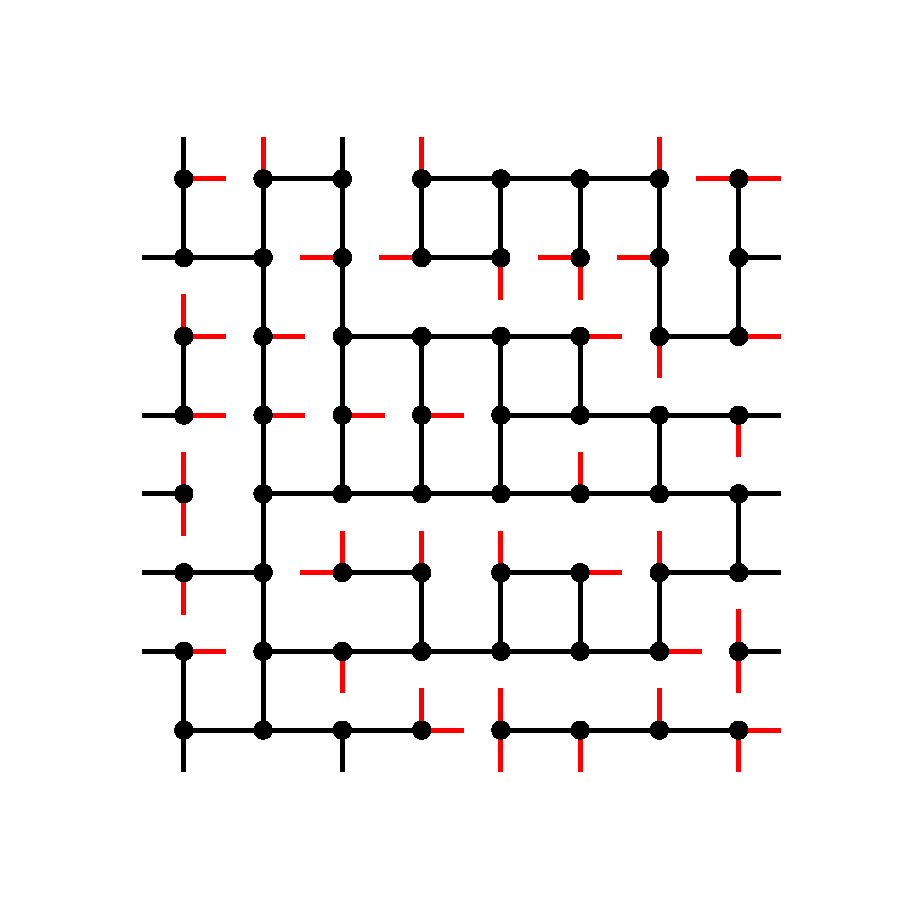
\includegraphics[width=\textwidth]{./figures/procrystals/pro_mc_1.pdf}
         \caption{Initial random lattice.}
         \label{fig:promca}
     \end{subfigure}
     \hfill
     \begin{subfigure}[b]{0.3\textwidth}
         \centering
         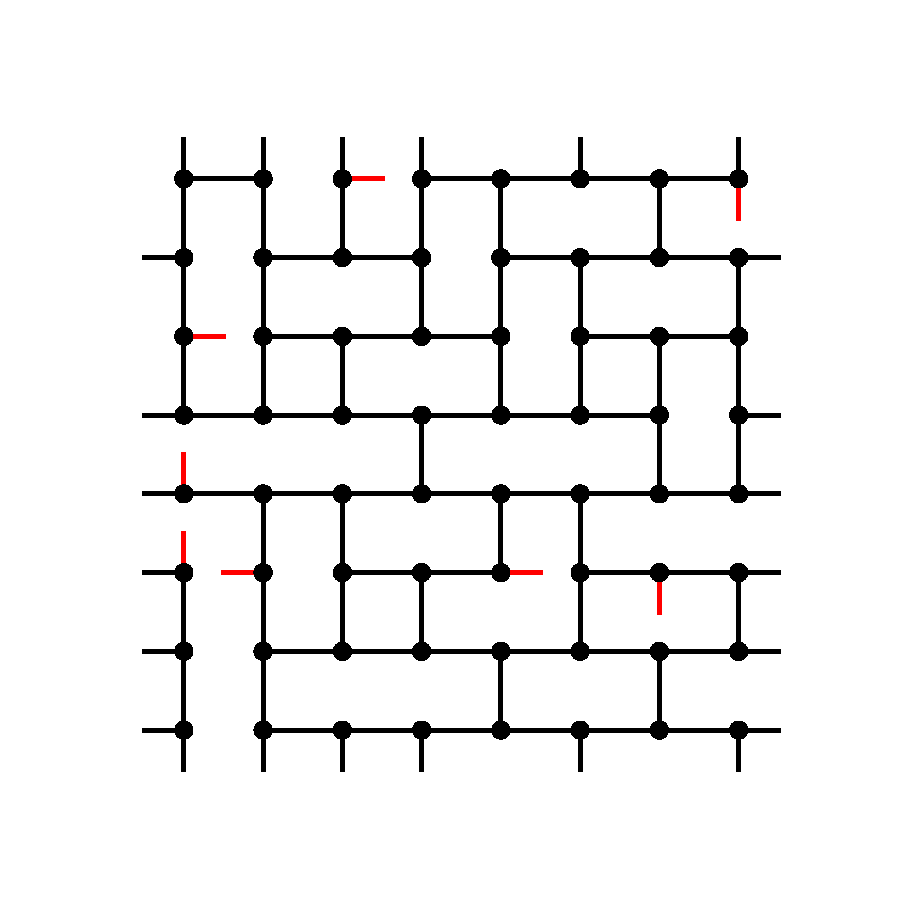
\includegraphics[width=\textwidth]{./figures/procrystals/pro_mc_3.pdf}
         \caption{Partial convergence.}
         \label{fig:promcb}
     \end{subfigure}
     \hfill
     \begin{subfigure}[b]{0.3\textwidth}
         \centering
         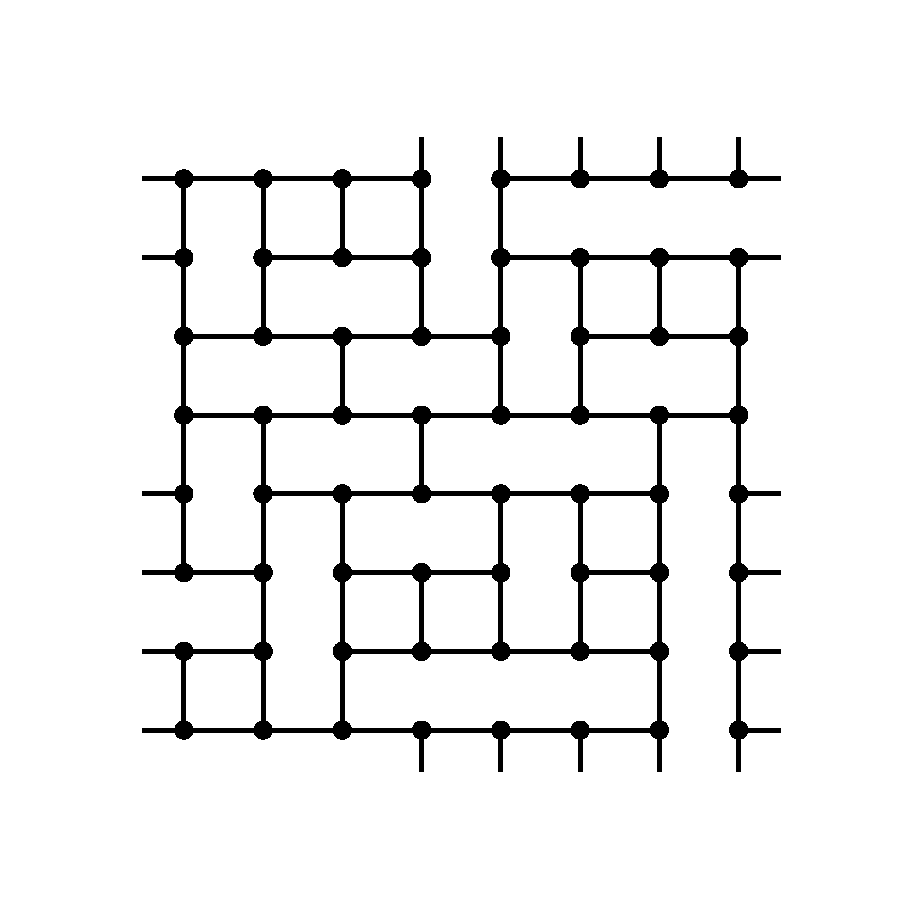
\includegraphics[width=\textwidth]{./figures/procrystals/pro_mc_4.pdf}
         \caption{Procrystalline lattice.}
         \label{fig:promcc}
     \end{subfigure}
     \hfill
     
     \caption{Stages in the \mc{} search for \pro{4}{3}square procrystalline lattices. Panel (a) gives the initial lattice where each node has 3 bonds in random orientations, panel (b) a snapshot during the search where dangling bonds are being removed and panel (c) the final lattice. Satisfied bonds are coloured black and dangling bonds red.}
     \label{fig:promc}
\end{figure}

\section{Structure of 3\--Coordinate Procrystals}

The bulk of the investigation in this chapter will focus on \pro{c^\prime}{3}procrystalline lattices. 
As stated before, this is because such systems are most prevalent in nature and draw the most parallels with previous work. 
To study the ring structure of these procrystals, the \mc{} method detailed in \davidnote{ref} was used to generate configurations for each of the five underlying lattice types, with number of nodes in the lattice scaled to explore system size effects.
For each set of parameters some $100,000$ periodic procrystalline lattices were generated.
A visualisation of an example configuration based on each parent lattice type is given in figure \ref{fig:pro3} for reference. 
These configurations highlight some important features of the specific procrystalline lattices which will will be a useful for the coming discussions.

\begin{itemize}
	\item $\mathbf{4,3-}$\textbf{square}: only contains even\--membered rings in the set $k\in\left\{4,6,8\cdots\right\}$. The results from the lack of ``cross'' bonds (acting between opposite corners of a square). Rings must be linear as any ``L''\--shapes would require stabilisation of a $2$\--coordinate site. 
	\item $\mathbf{4,3-}$\textbf{trihexagonal}: is yet more constrained, containing only rings in the set $k=\left\{3,6,7,8,9\right\}$. Each ``large'' ring ($k>3$) is surrounded by $k-6$ triangles.
	\item $\mathbf{5,3-}$\textbf{elongated\--triangular}: difference between underlying and procrystalline lattice is now $2$ and the full ring size range is accessible $k\in\left\{3,4,5\dots\right\}$.
	\item $\mathbf{5,3-}$\textbf{snub\--square}: as above.
	\item $\mathbf{6,3-}$\textbf{triangular}: difference between underlying and procrystalline lattice is now $3$ and again $k\in\left\{3,4,5\dots\right\}$.	
\end{itemize}

\begin{figure}[bt]
     \centering
     
     \begin{subfigure}[b]{0.4\textwidth}
         \centering
         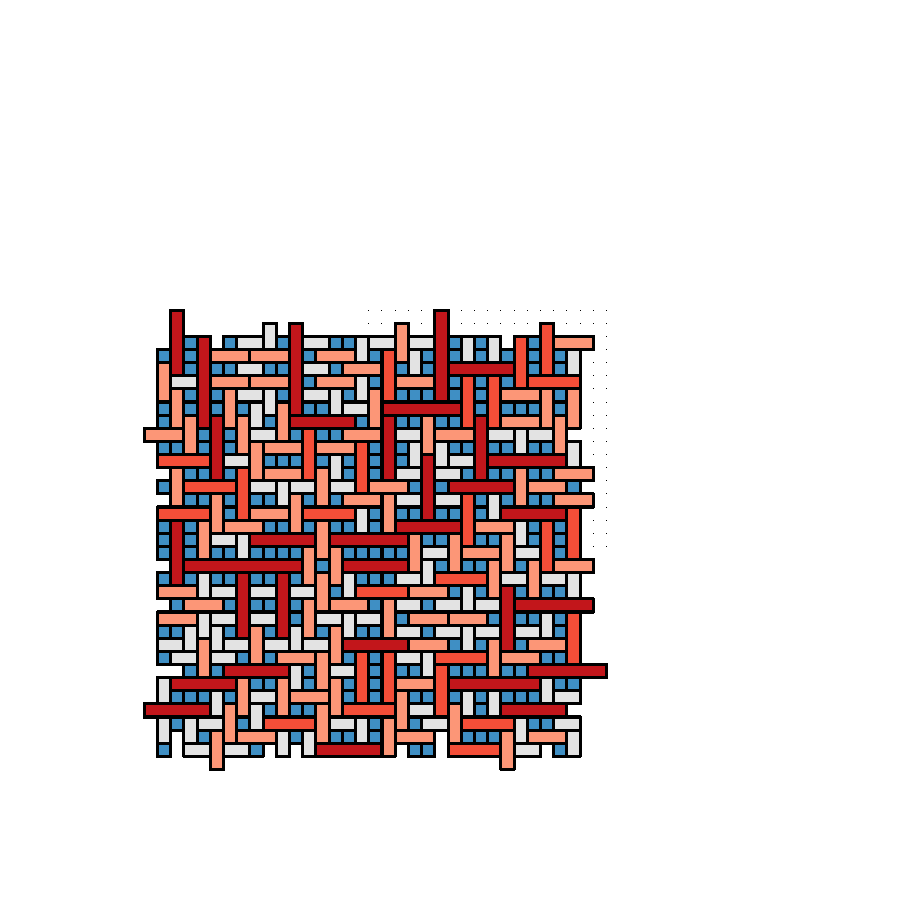
\includegraphics[height=4.5cm]{./figures/procrystals/pro_sq3.pdf}
         \caption{\pro{4}{3}square}
         \label{fig:pro3a}
     \end{subfigure}
      \begin{subfigure}[b]{0.45\textwidth}
         \centering
         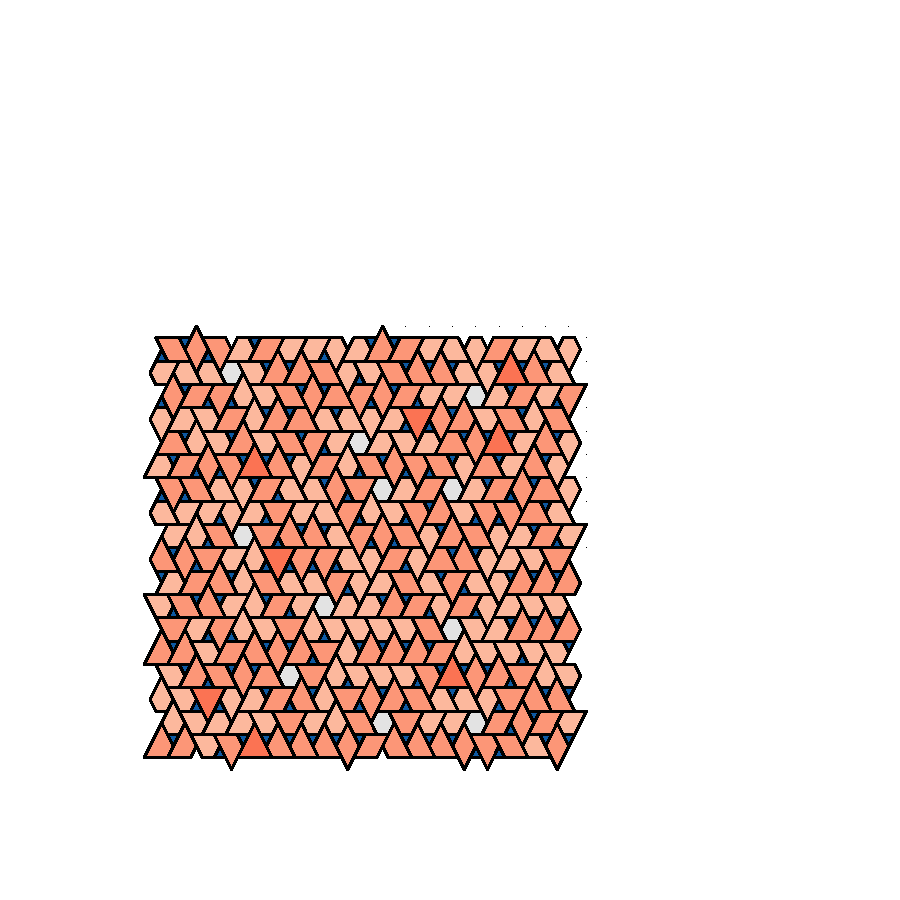
\includegraphics[height=4.5cm]{./figures/procrystals/pro_trihex3.pdf}
         \caption{\pro{4}{3}trihexagonal}
         \label{fig:pro3b}
     \end{subfigure}
     \hfill
     	
     \vspace{0.5cm}
     \begin{subfigure}[b]{0.3\textwidth}
         \centering
         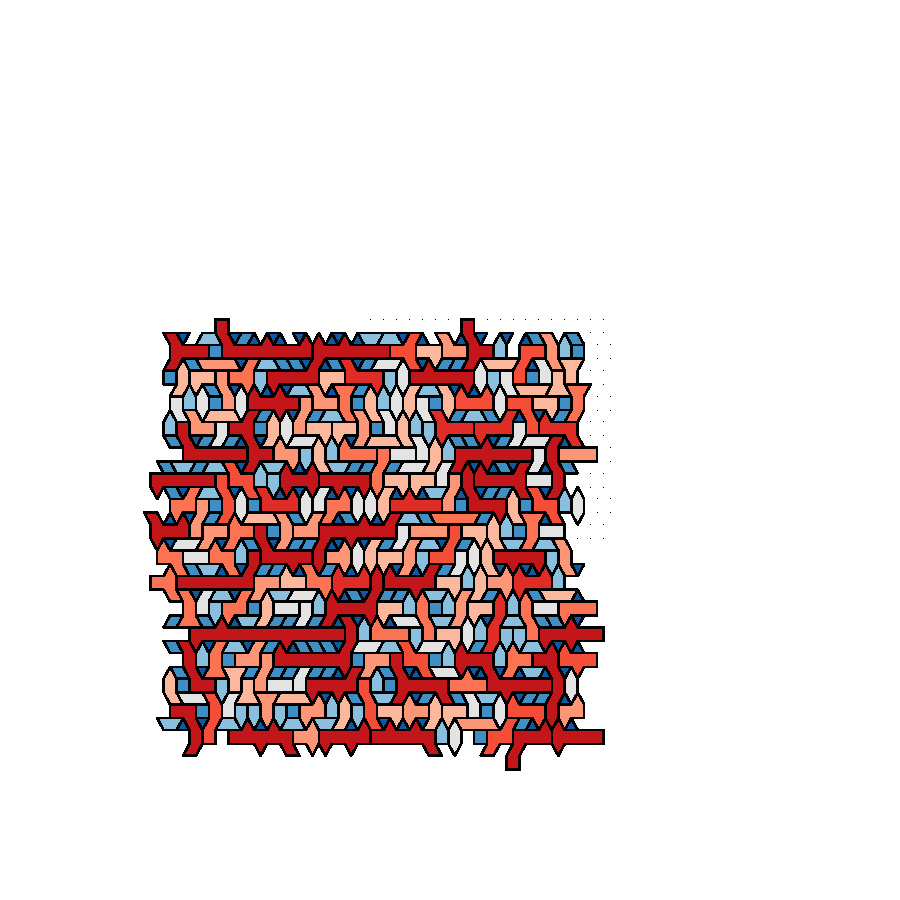
\includegraphics[height=4.5cm]{./figures/procrystals/pro_elong3.pdf}
         \caption{\pro{5}{3}elongated\--triangular}
         \label{fig:pro3c}
     \end{subfigure}
     \hfill
     \begin{subfigure}[b]{0.3\textwidth}
         \centering
         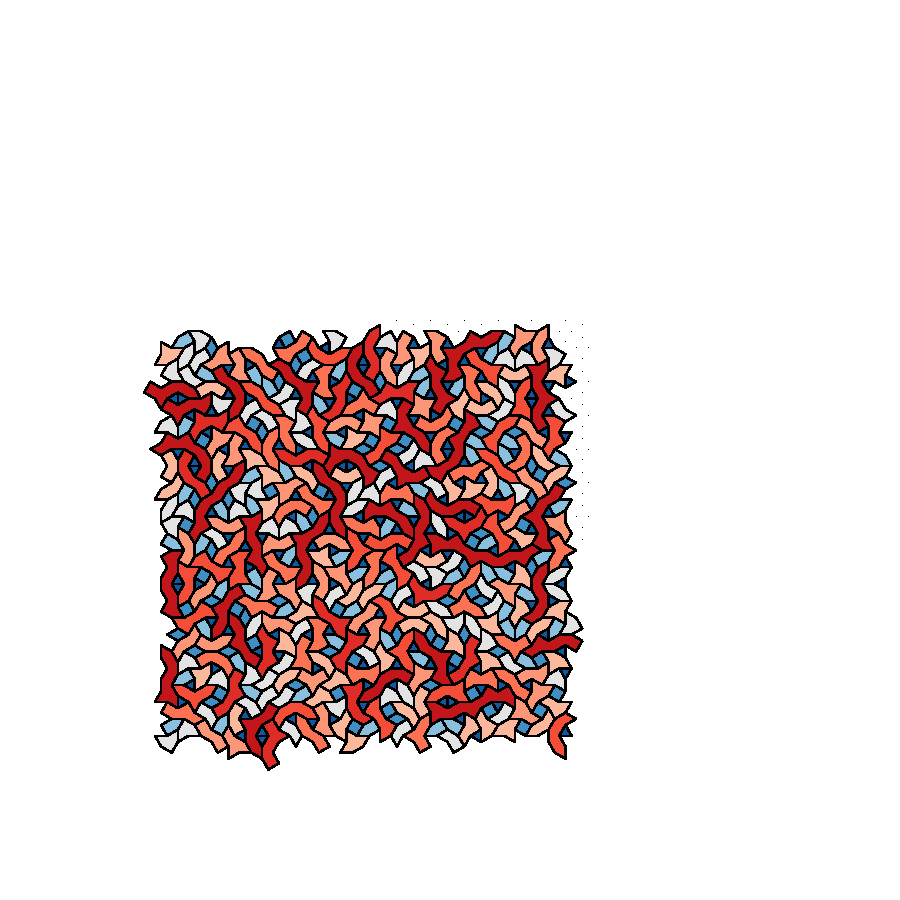
\includegraphics[height=4.5cm]{./figures/procrystals/pro_snub3.pdf}
         \caption{\pro{5}{3}snub\--square}
         \label{fig:pro3d}
     \end{subfigure}
     \hfill
     \begin{subfigure}[b]{0.3\textwidth}
         \centering
         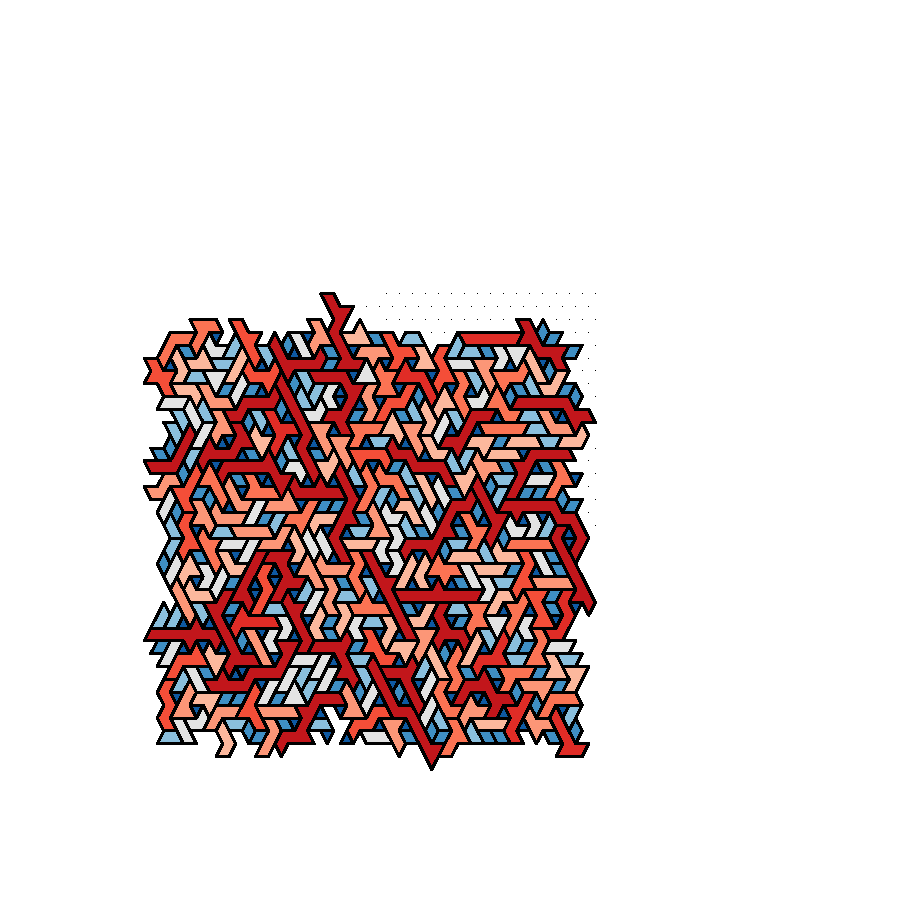
\includegraphics[height=4.5cm]{./figures/procrystals/pro_tri3.pdf}
         \caption{\pro{6}{3}triangular}
         \label{fig:pro3e}
     \end{subfigure}
     \hfill
    
     \caption{Visualisations of 3\--coordinate procrystals based on the 5 different parent lattices (as indicated in panel captions).}
     \label{fig:pro3}
\end{figure}

Importantly, these 3\--coordinate procrystals will be compared and contrasted with two other states.
The first are networks generated from bond switching at infinite temperature \davidnote{link}, which is in effect a method for producing continuous random networks (CRNs) \ie{} a fully amorphous state.
The second are crystals...



\subsection{Ring Size Distributions}